%!TEX root = index.tex
\section[Resultados]{Resultados}

\begin{frame}{Resultados}
\begin{table}[hp]
\begin{center}
    \caption{Parâmetros de influência no desempenho dos algoritmos de recomendação}\vspace{-.5cm}
    \label{tab:variaveis}
    \begin{tabular}{  | p{1.5cm} | p{5.5cm} | p{3.0cm} | } 
    \hline
    \textbf{Variável} & \textbf{Descrição} & \textbf{Valor padrão}  \\ \hline
    $N$ & Lista de recomendação & $20$ \\ \hline   
    $T$ & Base de treinamento & $75\%$ \\ \hline
    $H$ & Avaliações ``escondidas'' & $75\%$ \\ \hline
    $d^f$ & Medida de distância & Distância $L_1$~$\left|\left|\cdot\right|\right|^f$ \\ \hline
    $\mathcal{F}$ & Conjunto de atributos dos itens & Todos atributos \\ \hline
    $M$ & Avaliações positivas & $2$ \\ \hline
    $k$ & Vizinhos mais próximos & $10$ \\ \hline
    $W$ & Quantidade de pesos & Todo $w_f>0$ \\ \hline
    \end{tabular}
\end{center}
\end{table}
\end{frame}

\begin{frame}{Resultados}{Tamanho da lista de recomendação $N$}

\begin{columns}[b]
\column{.5\textwidth} %
\begin{figure}[ht]
    \begin{center}
    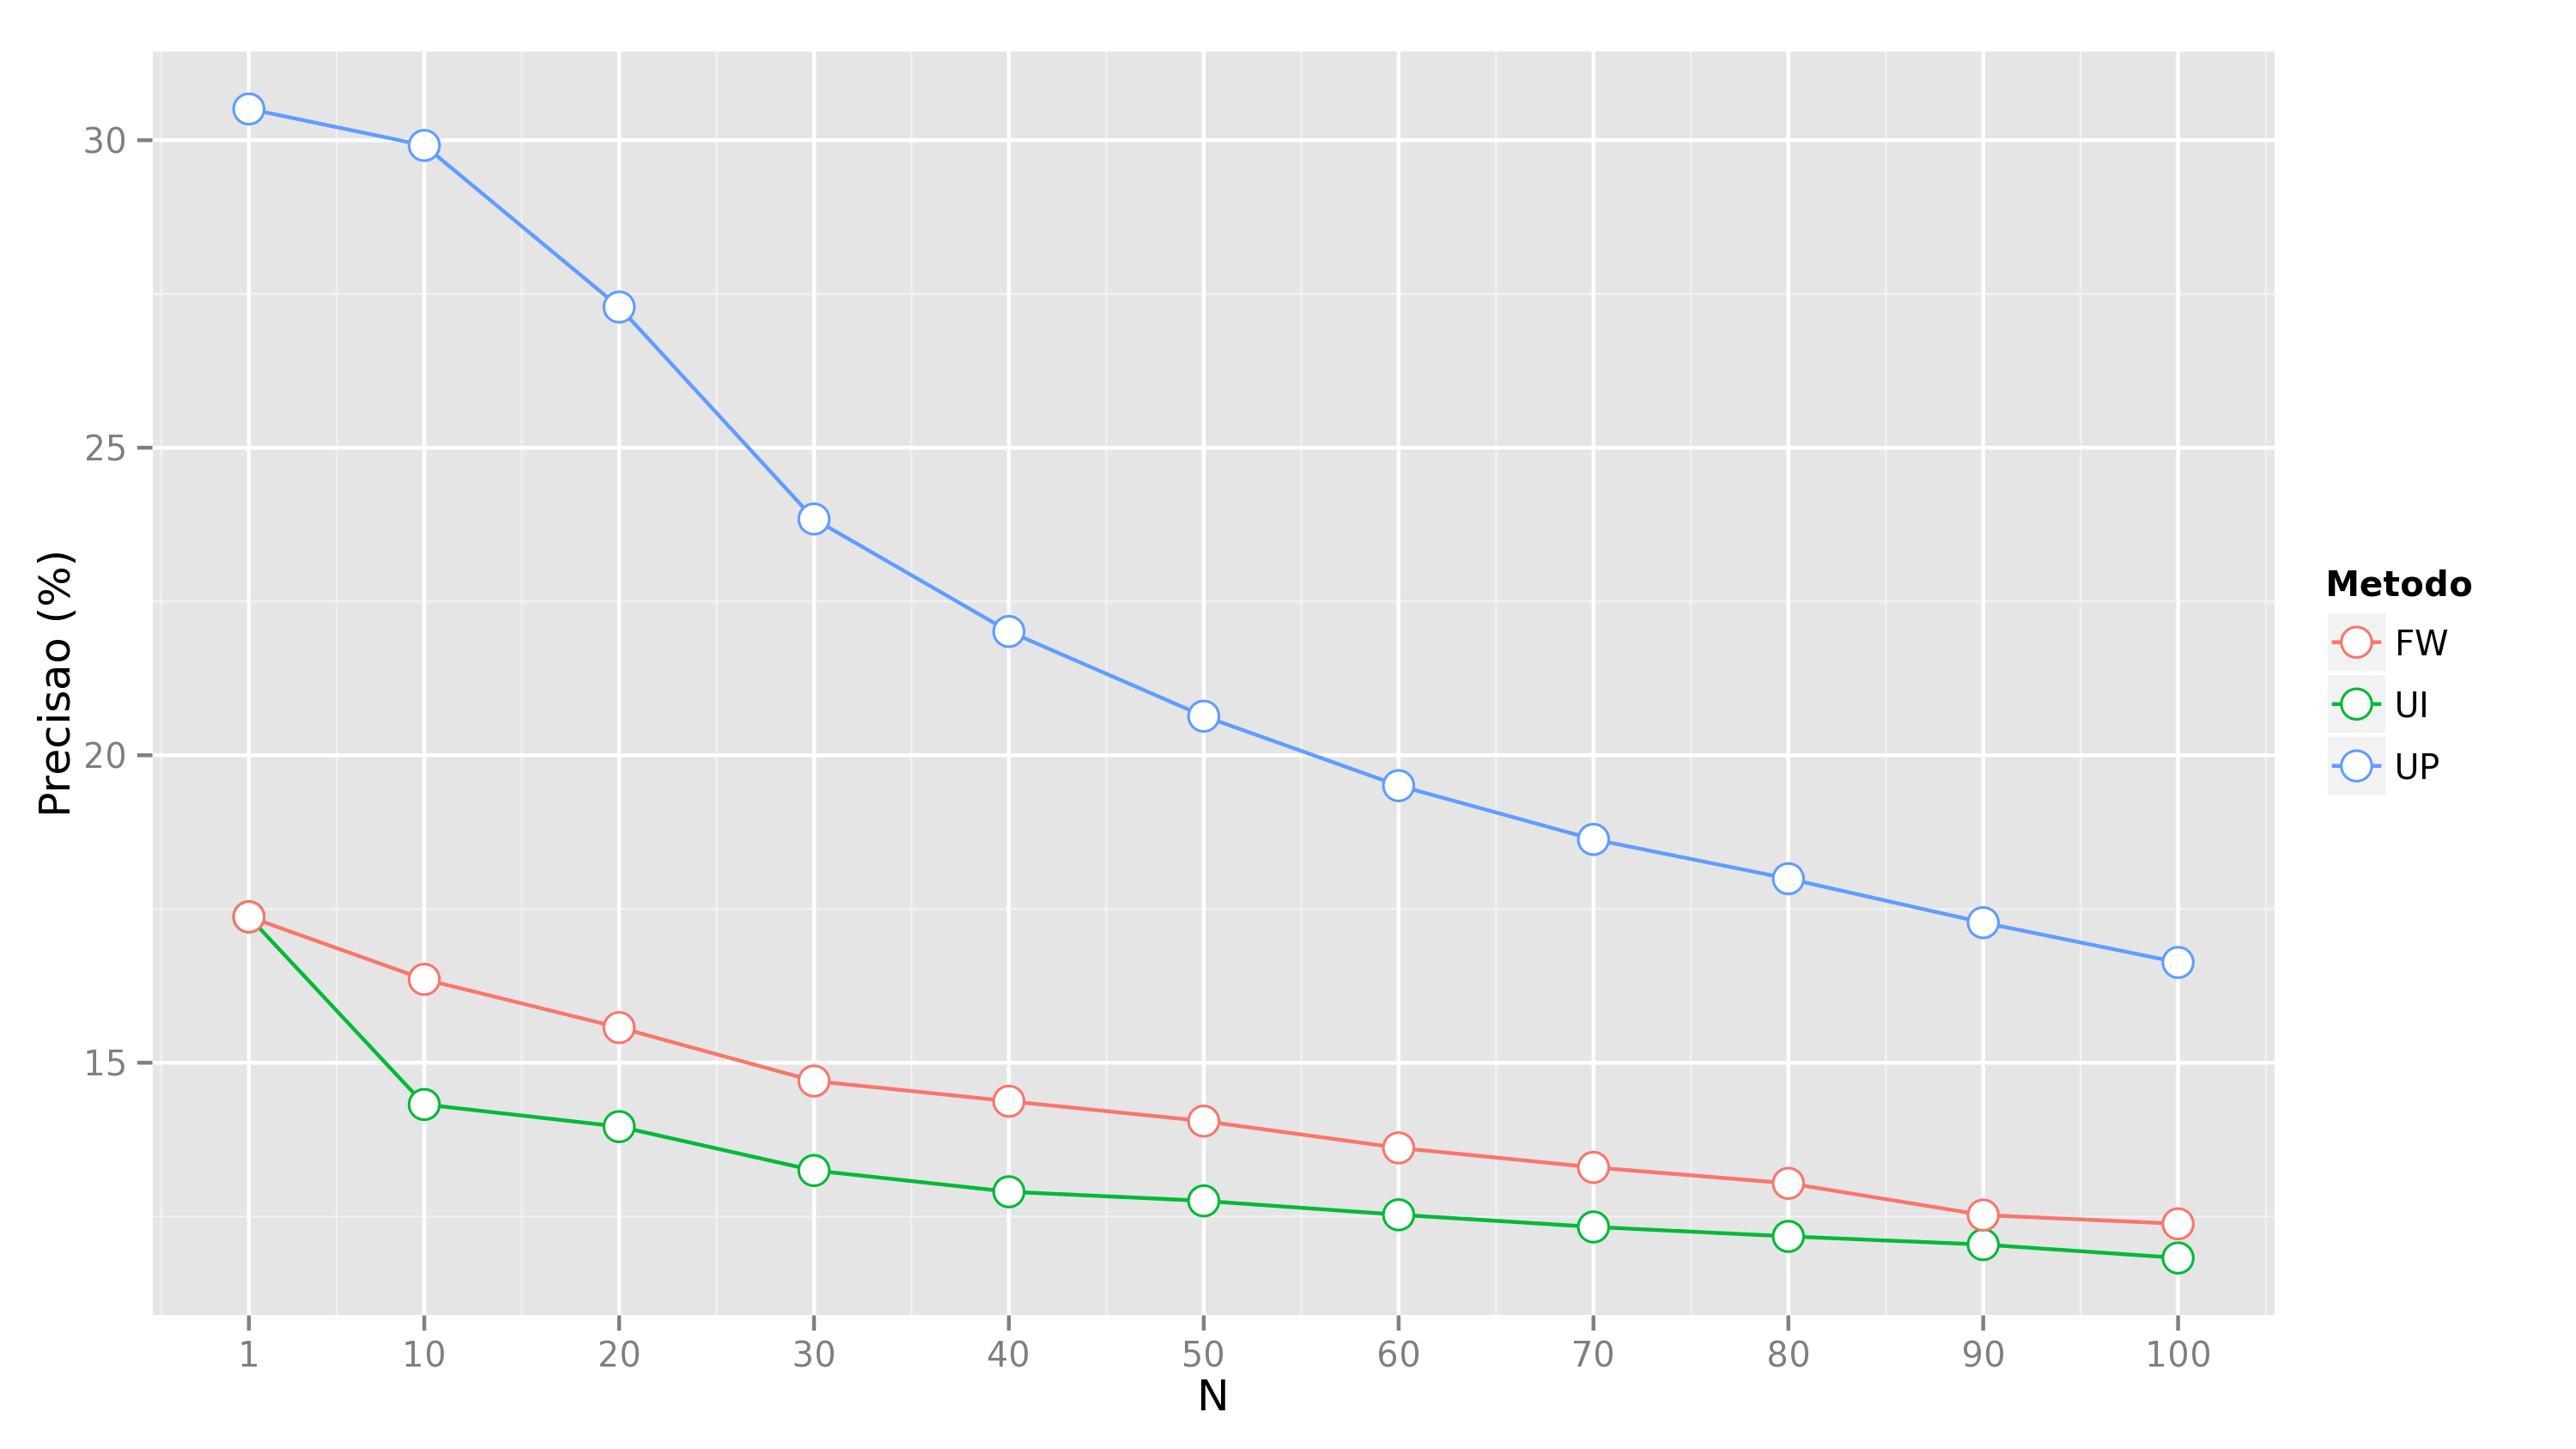
\includegraphics[width=1.1\textwidth]{../img/precision_N}
    \end{center}
    \caption{Precisão $\times$ $N$}
    \label{fig:precision_N}
\end{figure}

\column{.5\textwidth} % 

\begin{figure}[ht]
    \begin{center}
    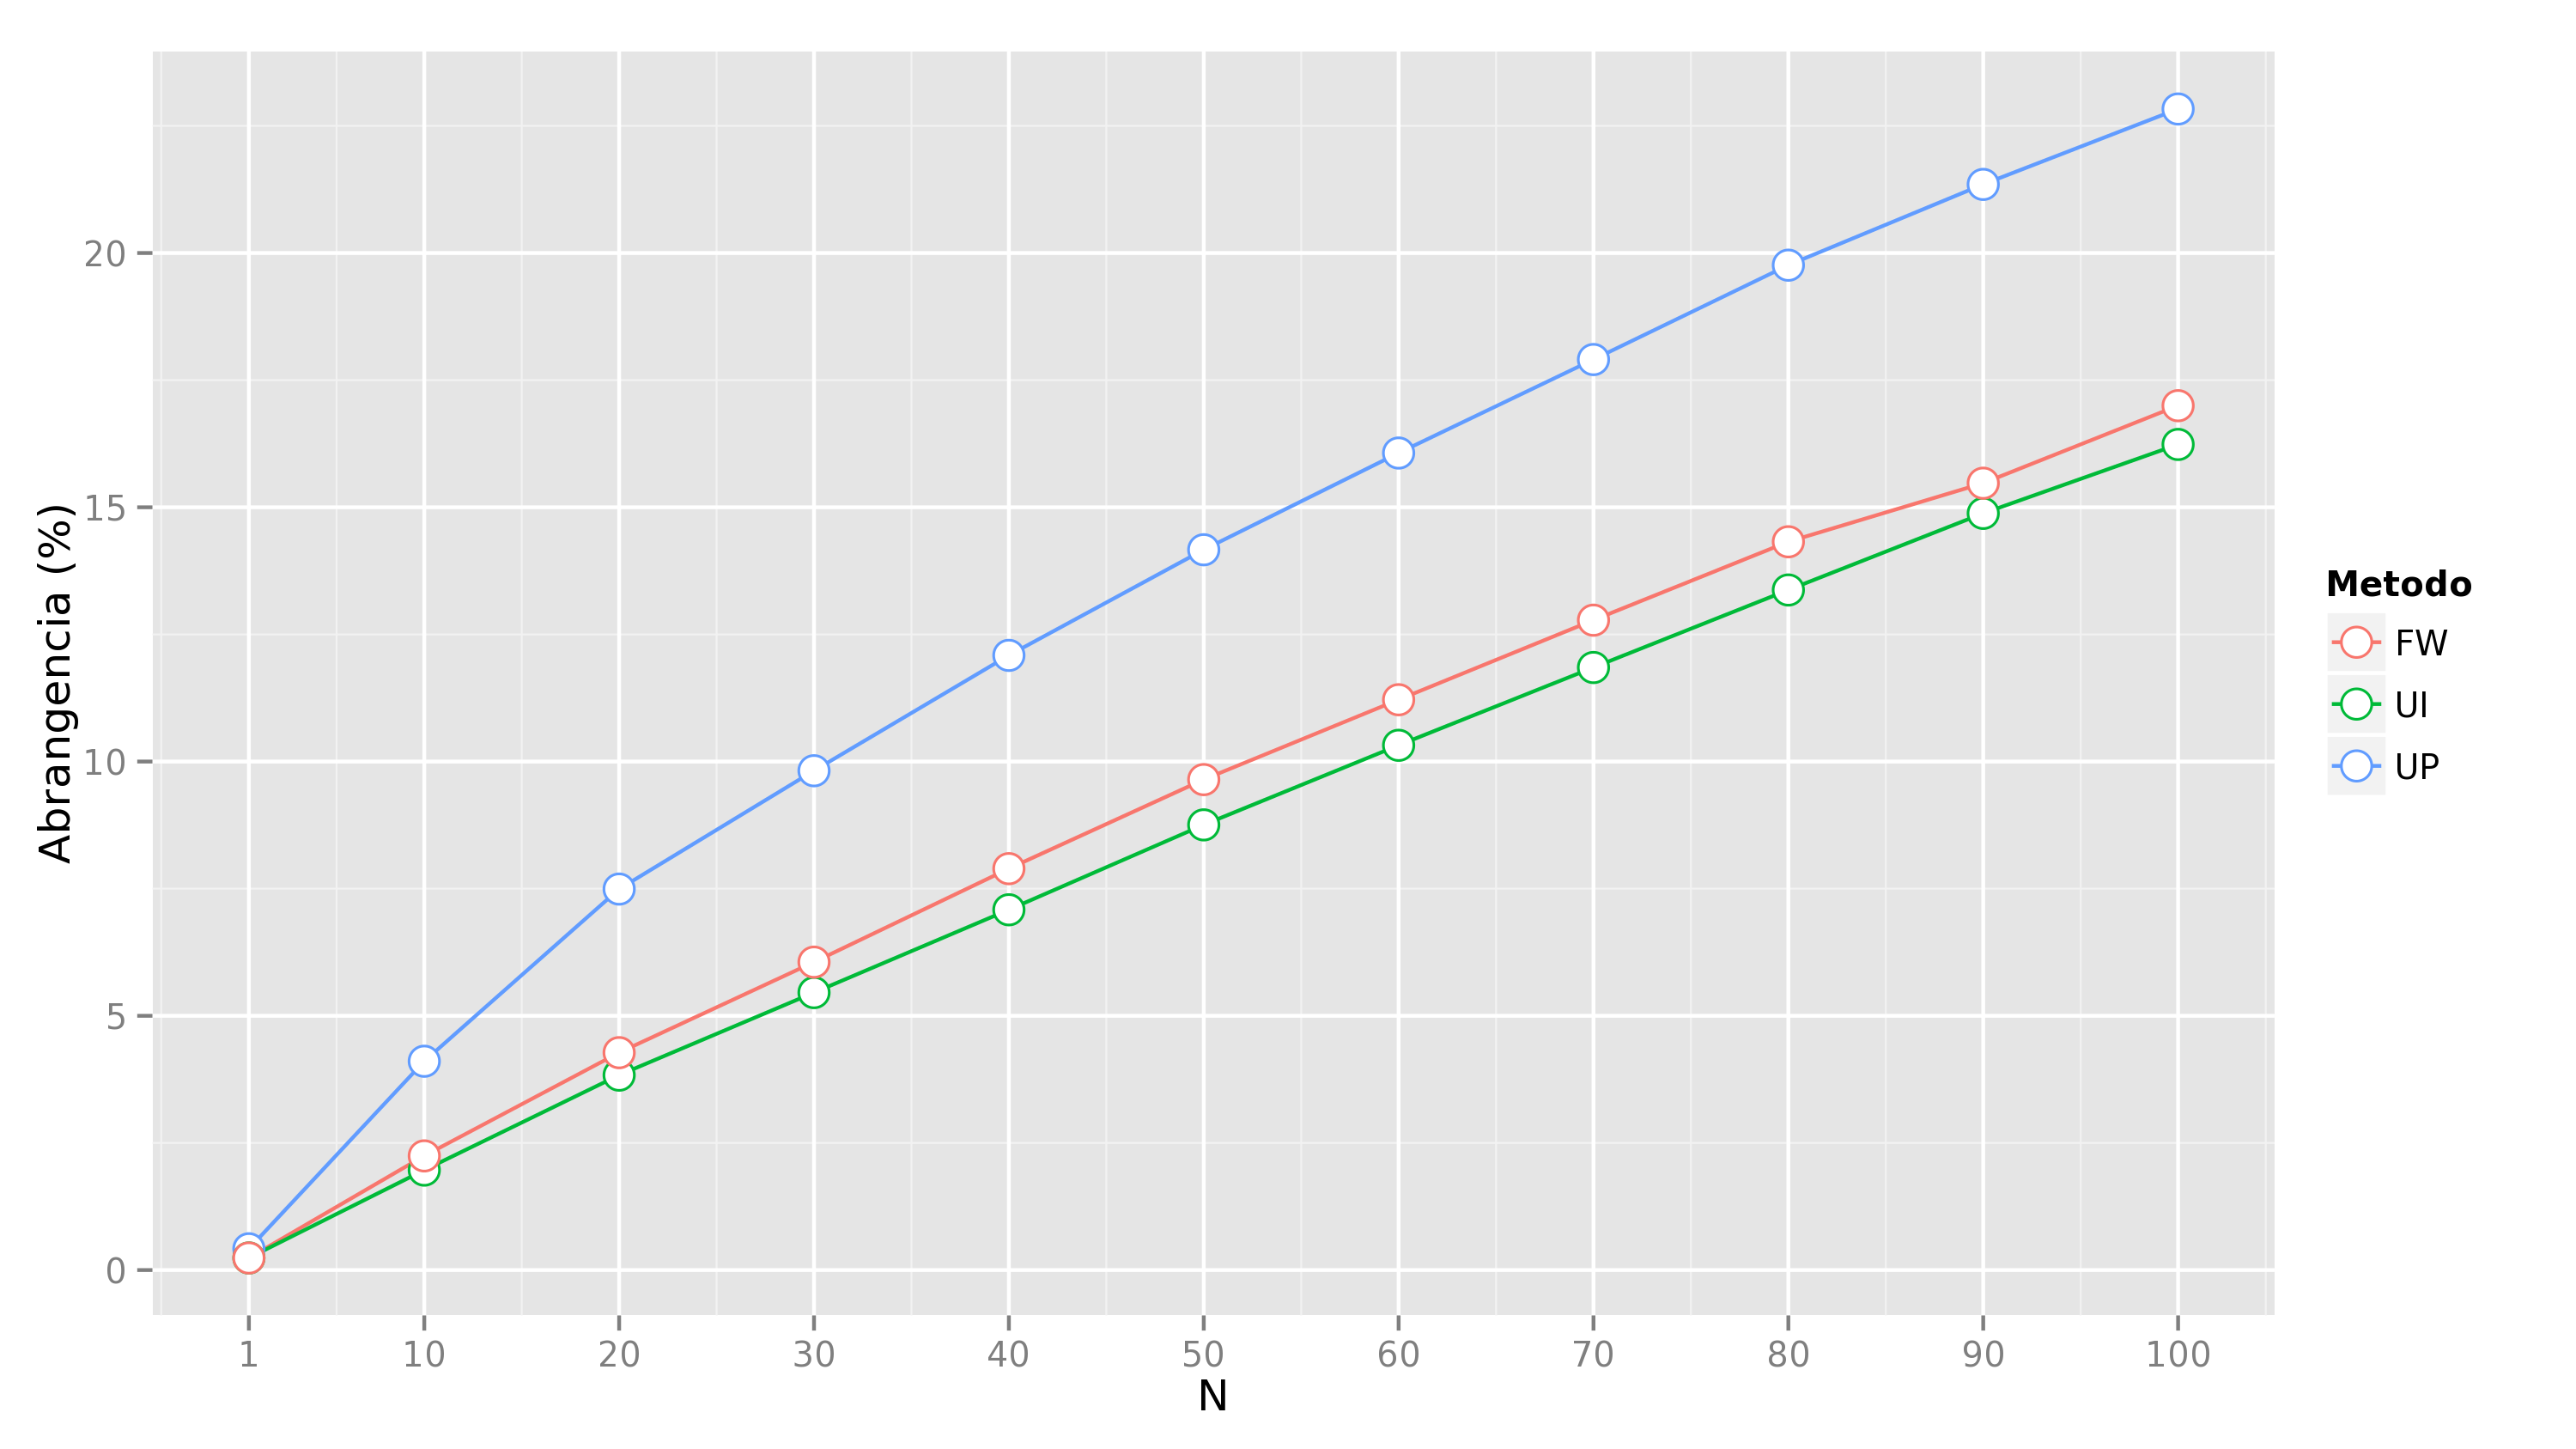
\includegraphics[width=1.1\textwidth]{../img/recall_N}
    \end{center}
    \caption{Abrangência $\times$ $N$}
    \label{fig:recall_N}
\end{figure}
\end{columns}
\end{frame}

\begin{frame}{Resultados}{Tamanho da lista de recomendação $N$}
\begin{columns}[b]
\column{.5\textwidth} %
\begin{figure}[ht]
    \begin{center}
    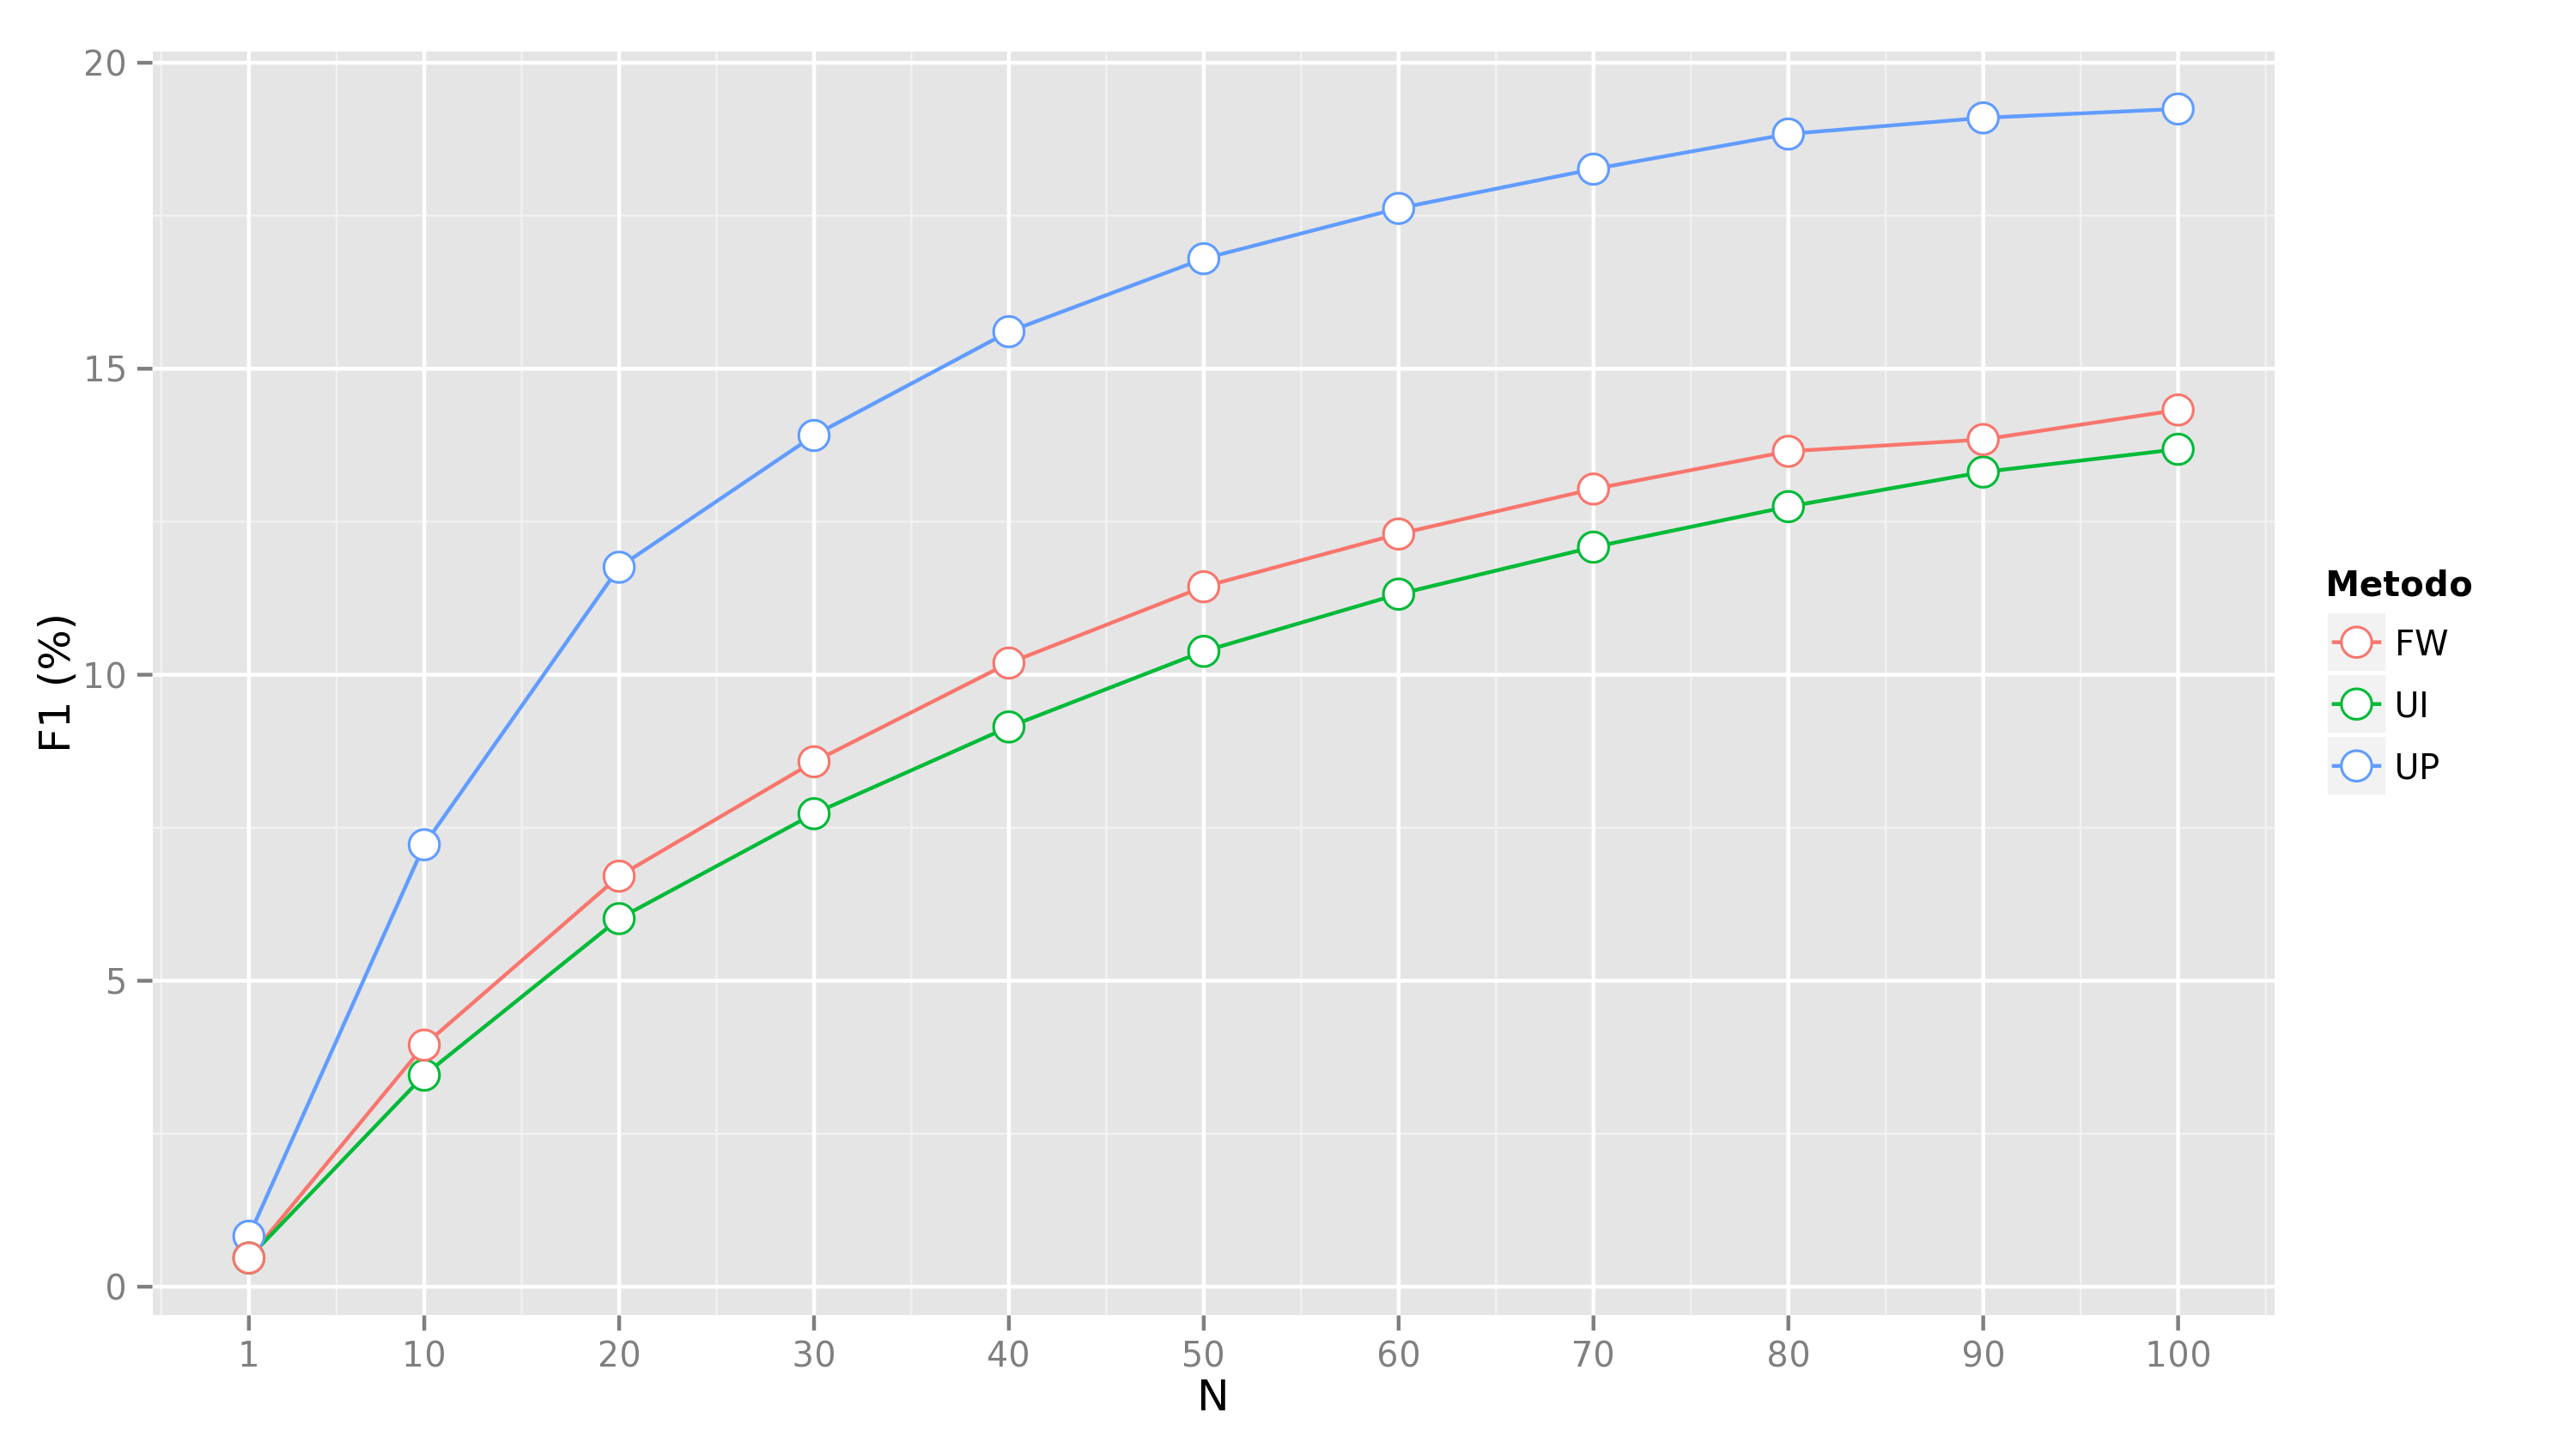
\includegraphics[width=1.1\textwidth]{../img/F1_N}
    \end{center}
    \caption{$F_1$ $\times$ $N$}
    \label{fig:F1_N}
\end{figure}

\column{.5\textwidth} % 

\begin{figure}[ht]
    \begin{center}
    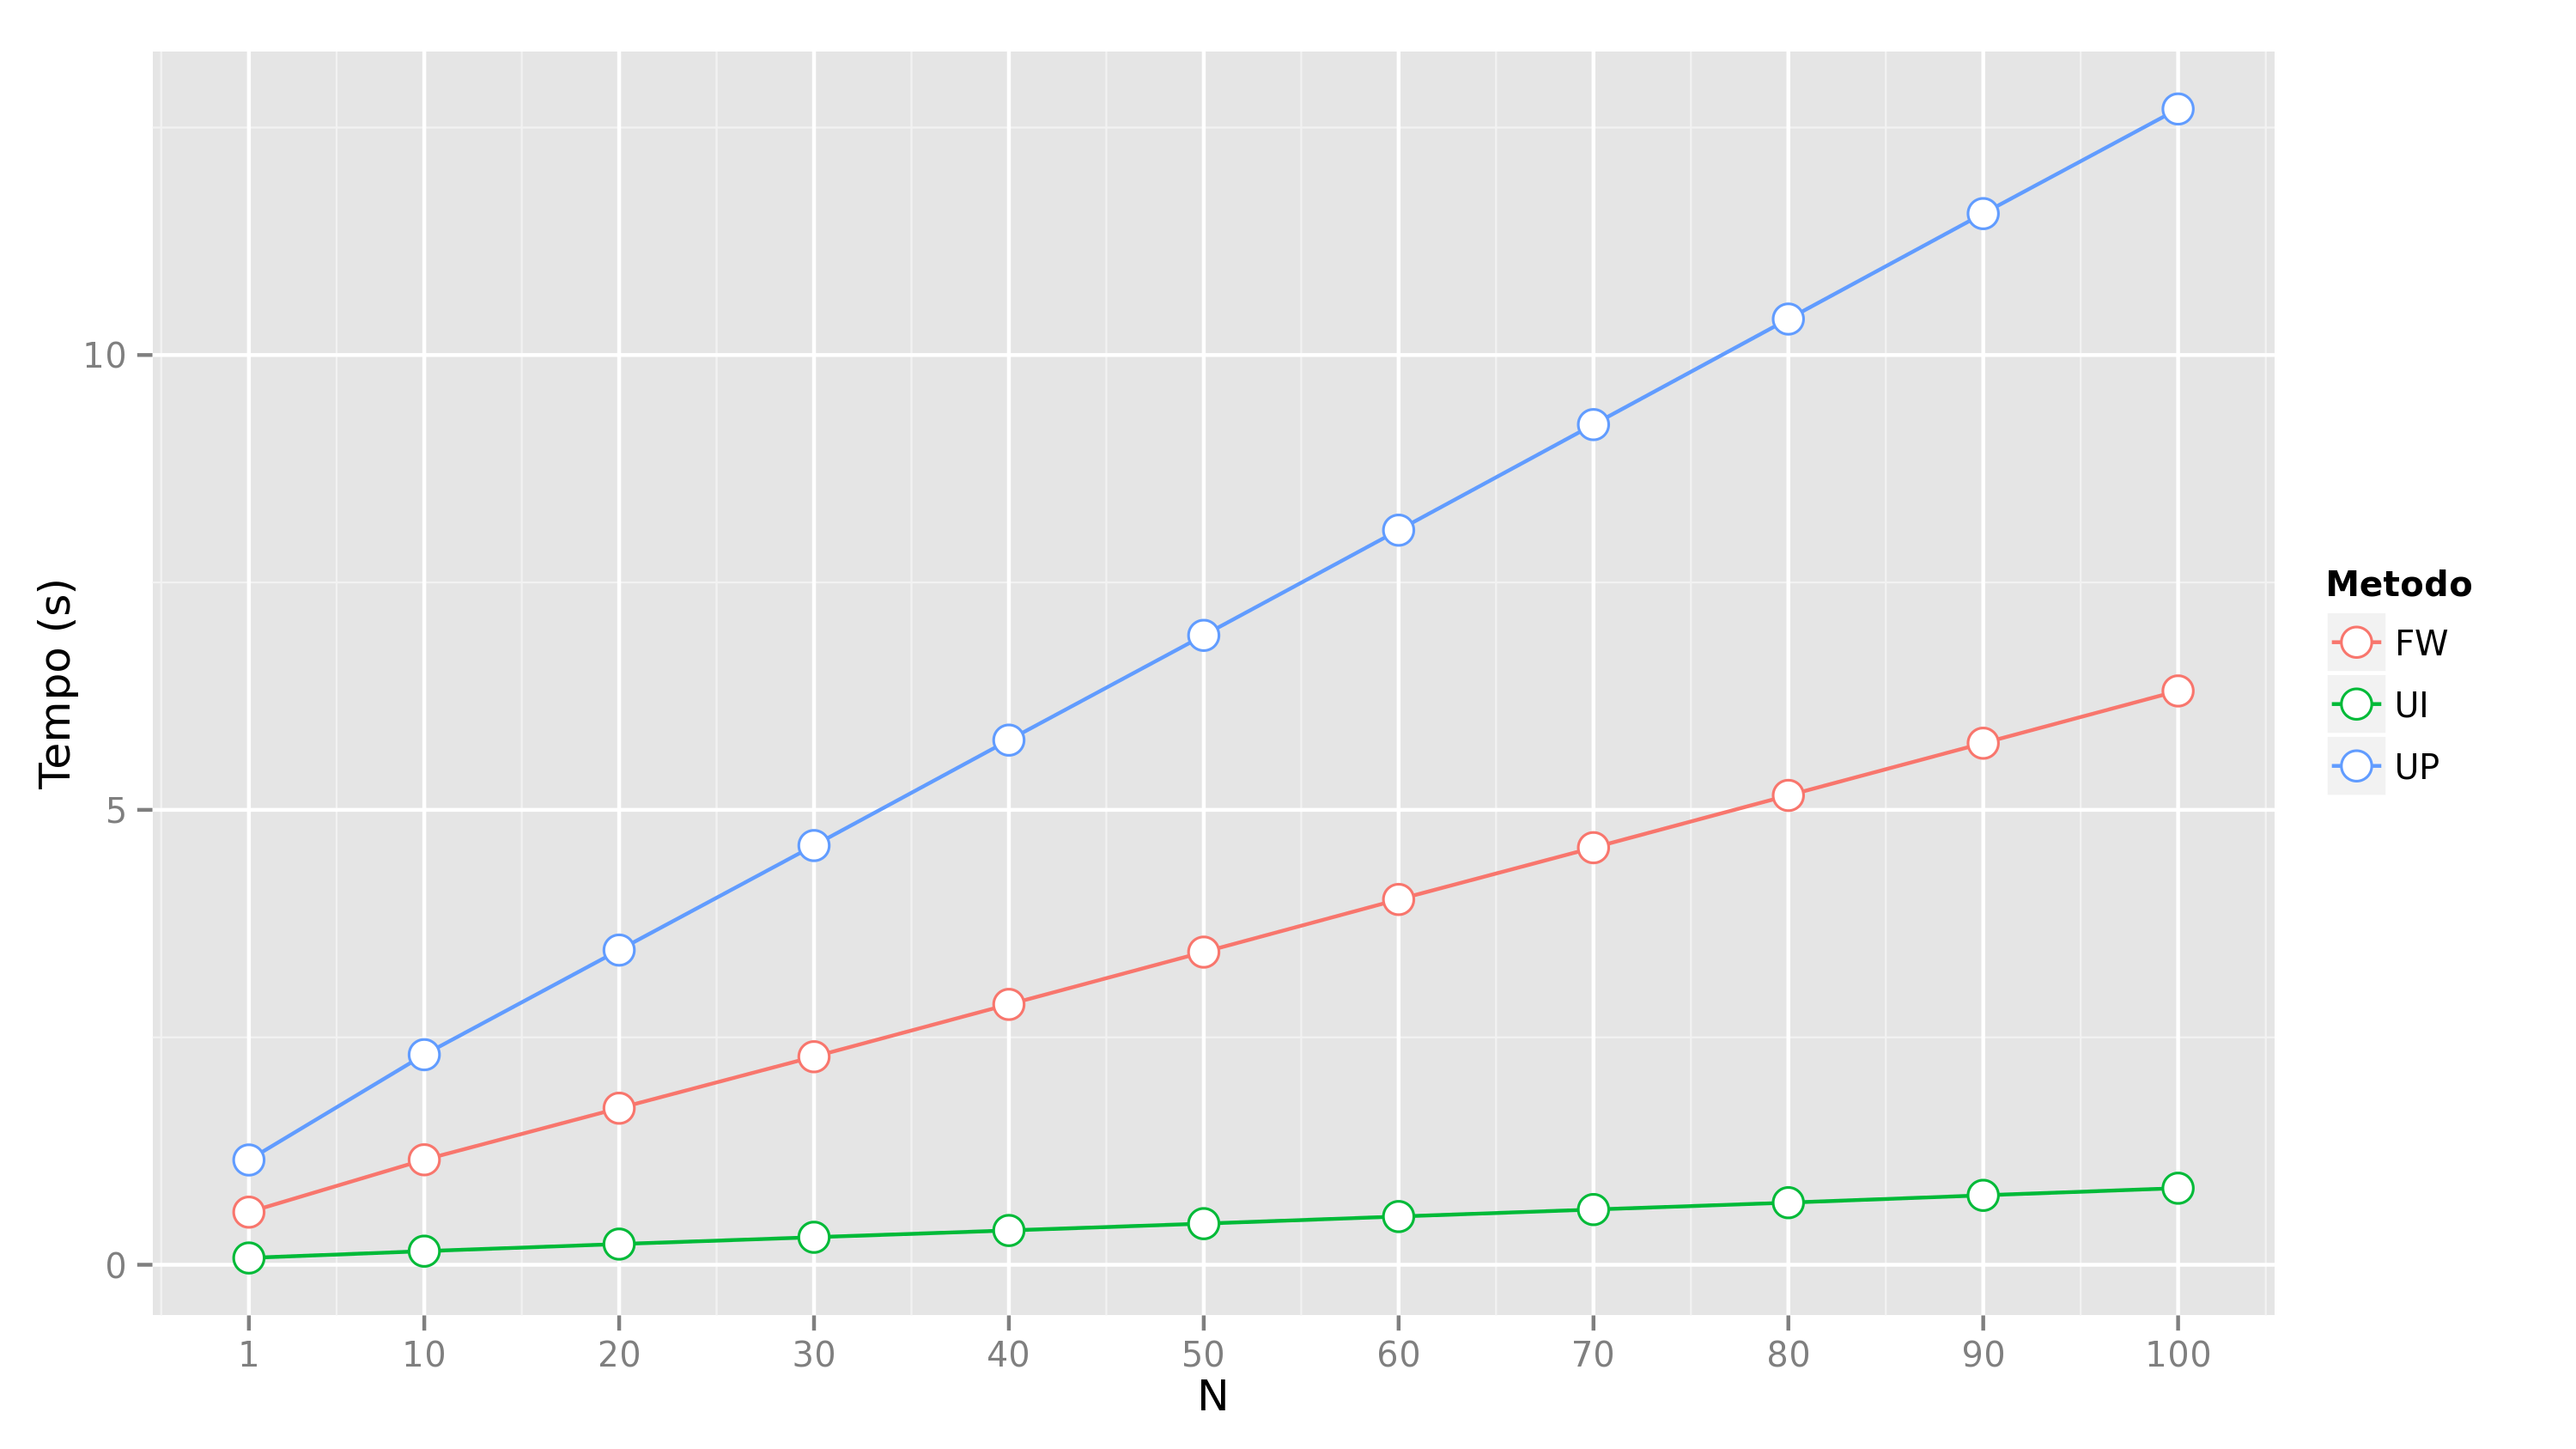
\includegraphics[width=1.1\textwidth]{../img/time_N}
    \end{center}
    \caption{Tempo $\times$ $N$}
    \label{fig:time_N}
\end{figure}
\end{columns}
\end{frame}

\begin{frame}{Resultados}{Percentual da base de aprendizado $T$}
\begin{figure}[ht]
    \begin{center}
    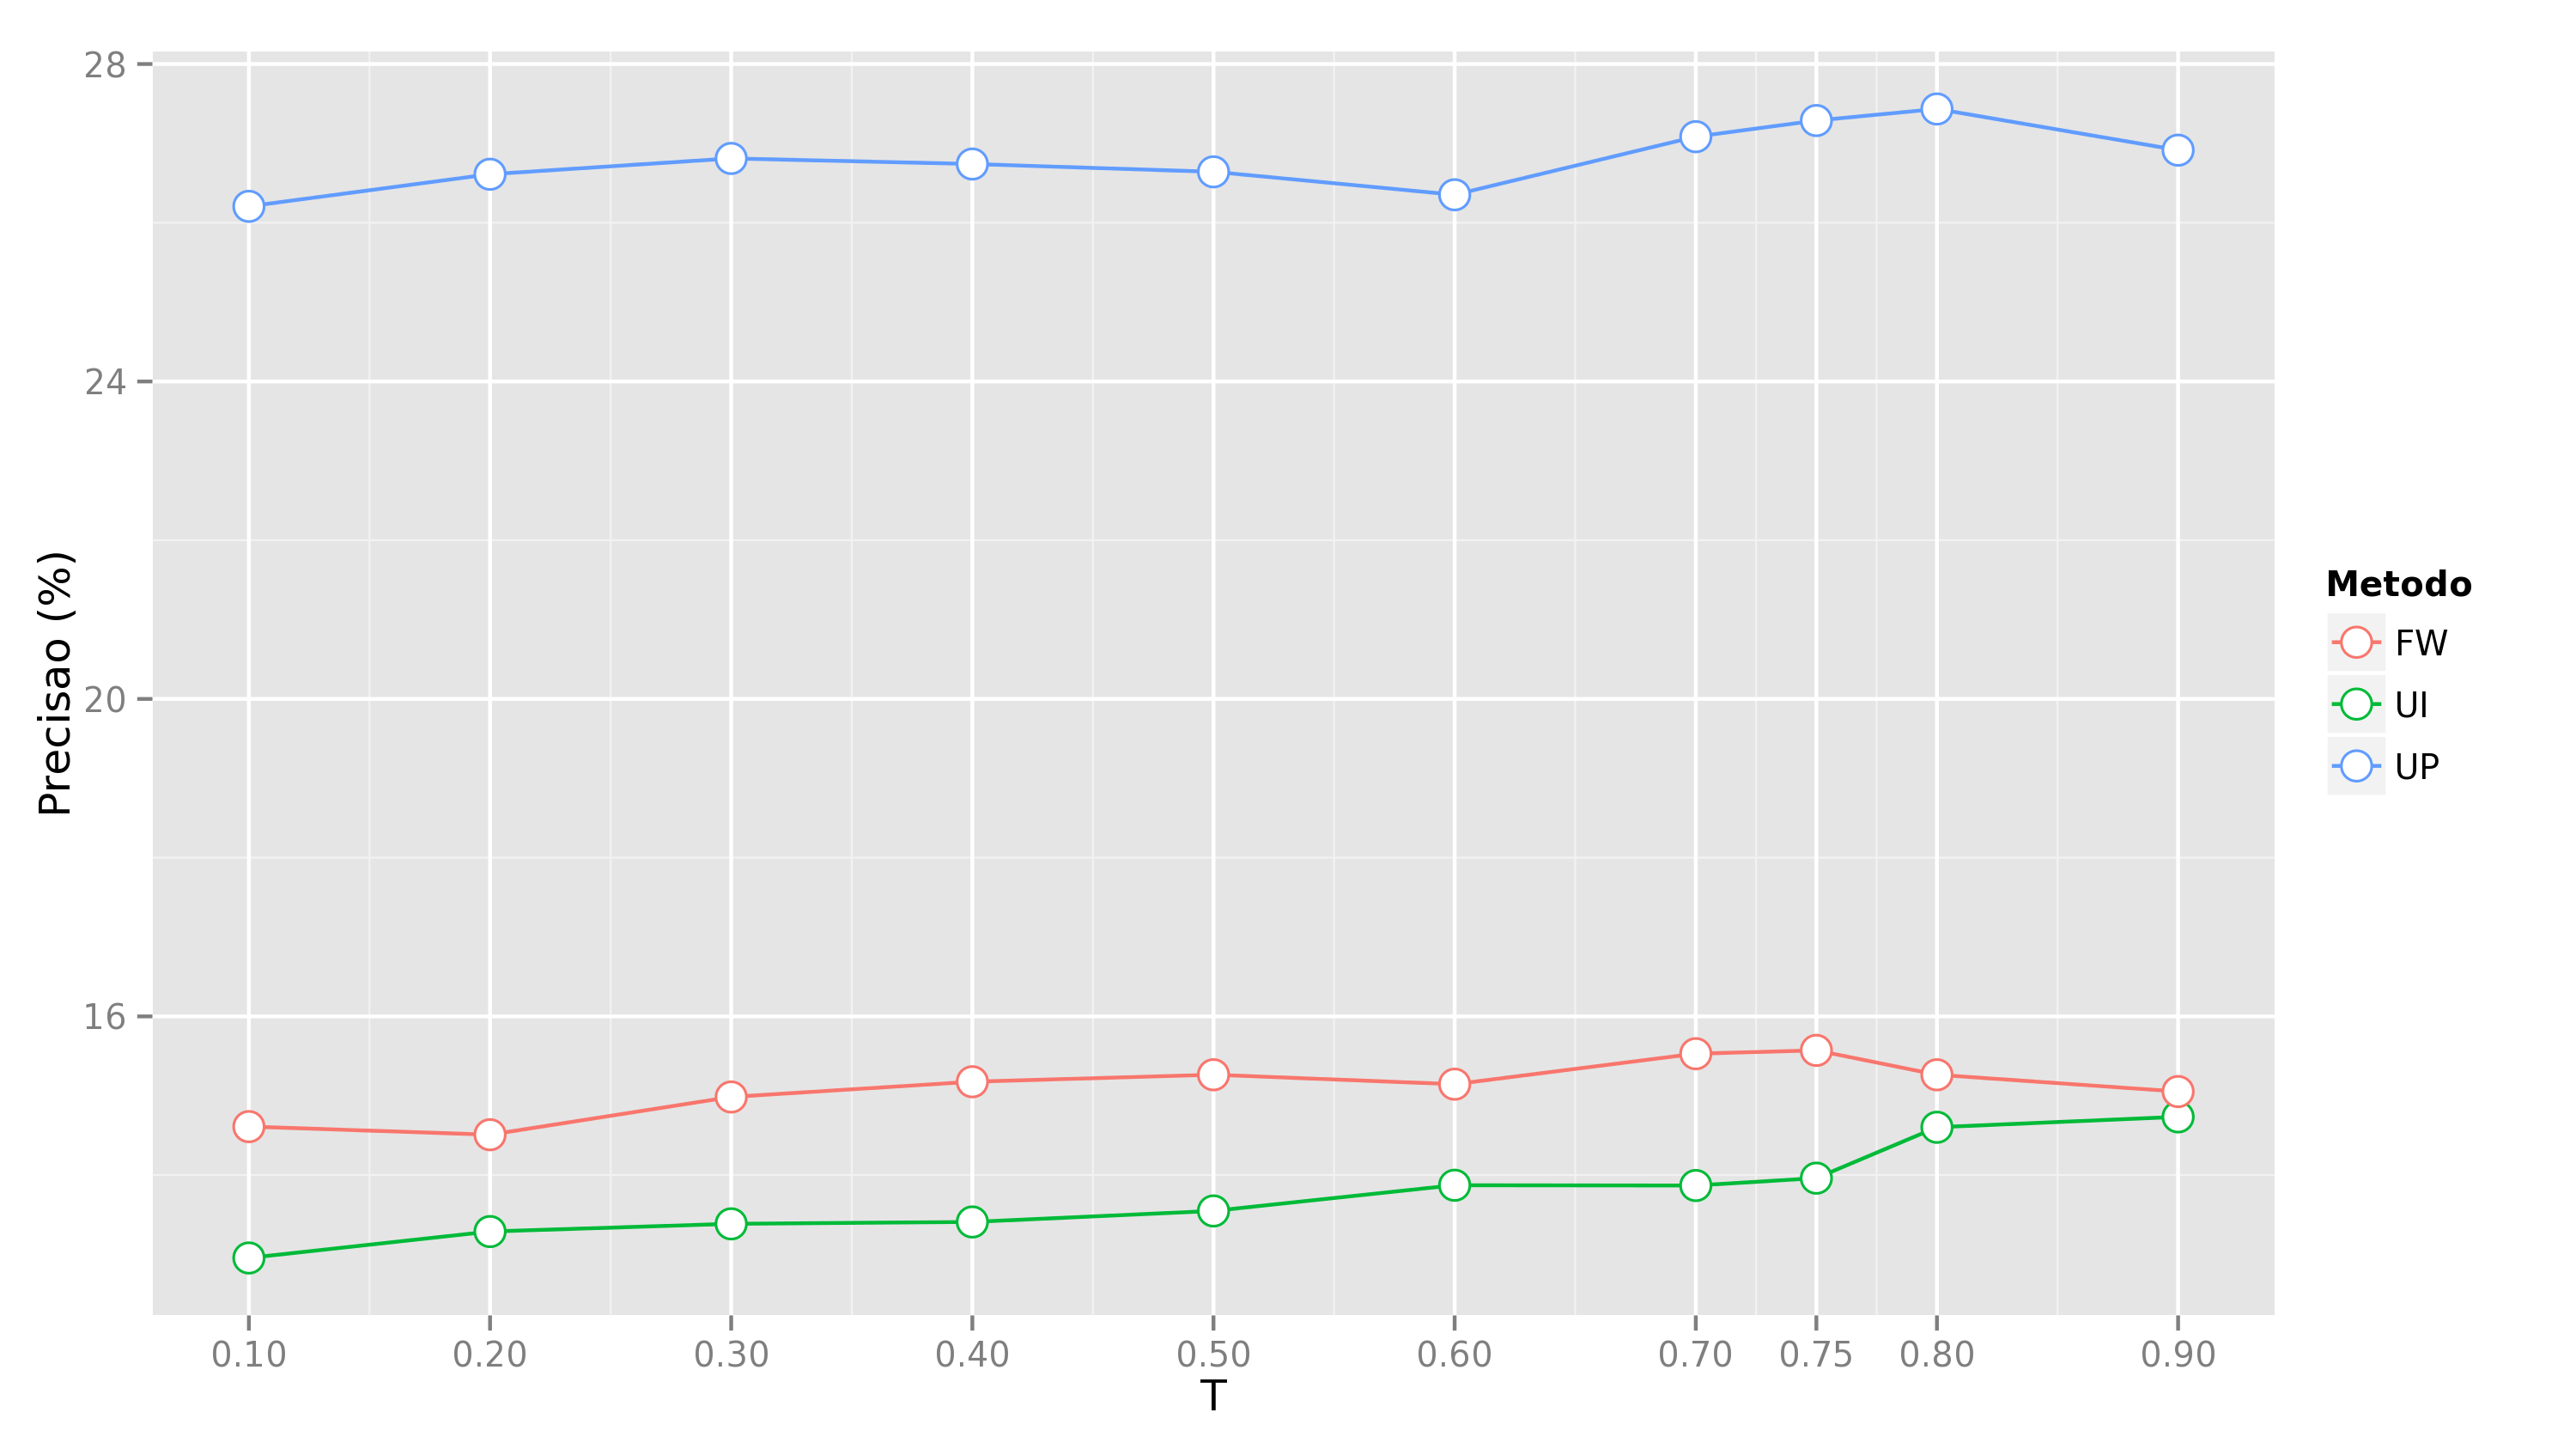
\includegraphics[width=.8\textwidth]{../img/precision_T}
    \end{center}
    \caption{Precisão $\times$ $T$}
    \label{fig:precision_T}
\end{figure}
\begin{center}
    Abrangência, $F_1$ e Tempo praticamente constantes
\end{center}
\end{frame}

\begin{frame}{Resultados}{Percentual de avaliações ``escondidas'' dos usuários-teste $H$}
\begin{figure}[ht]
    \begin{center}
    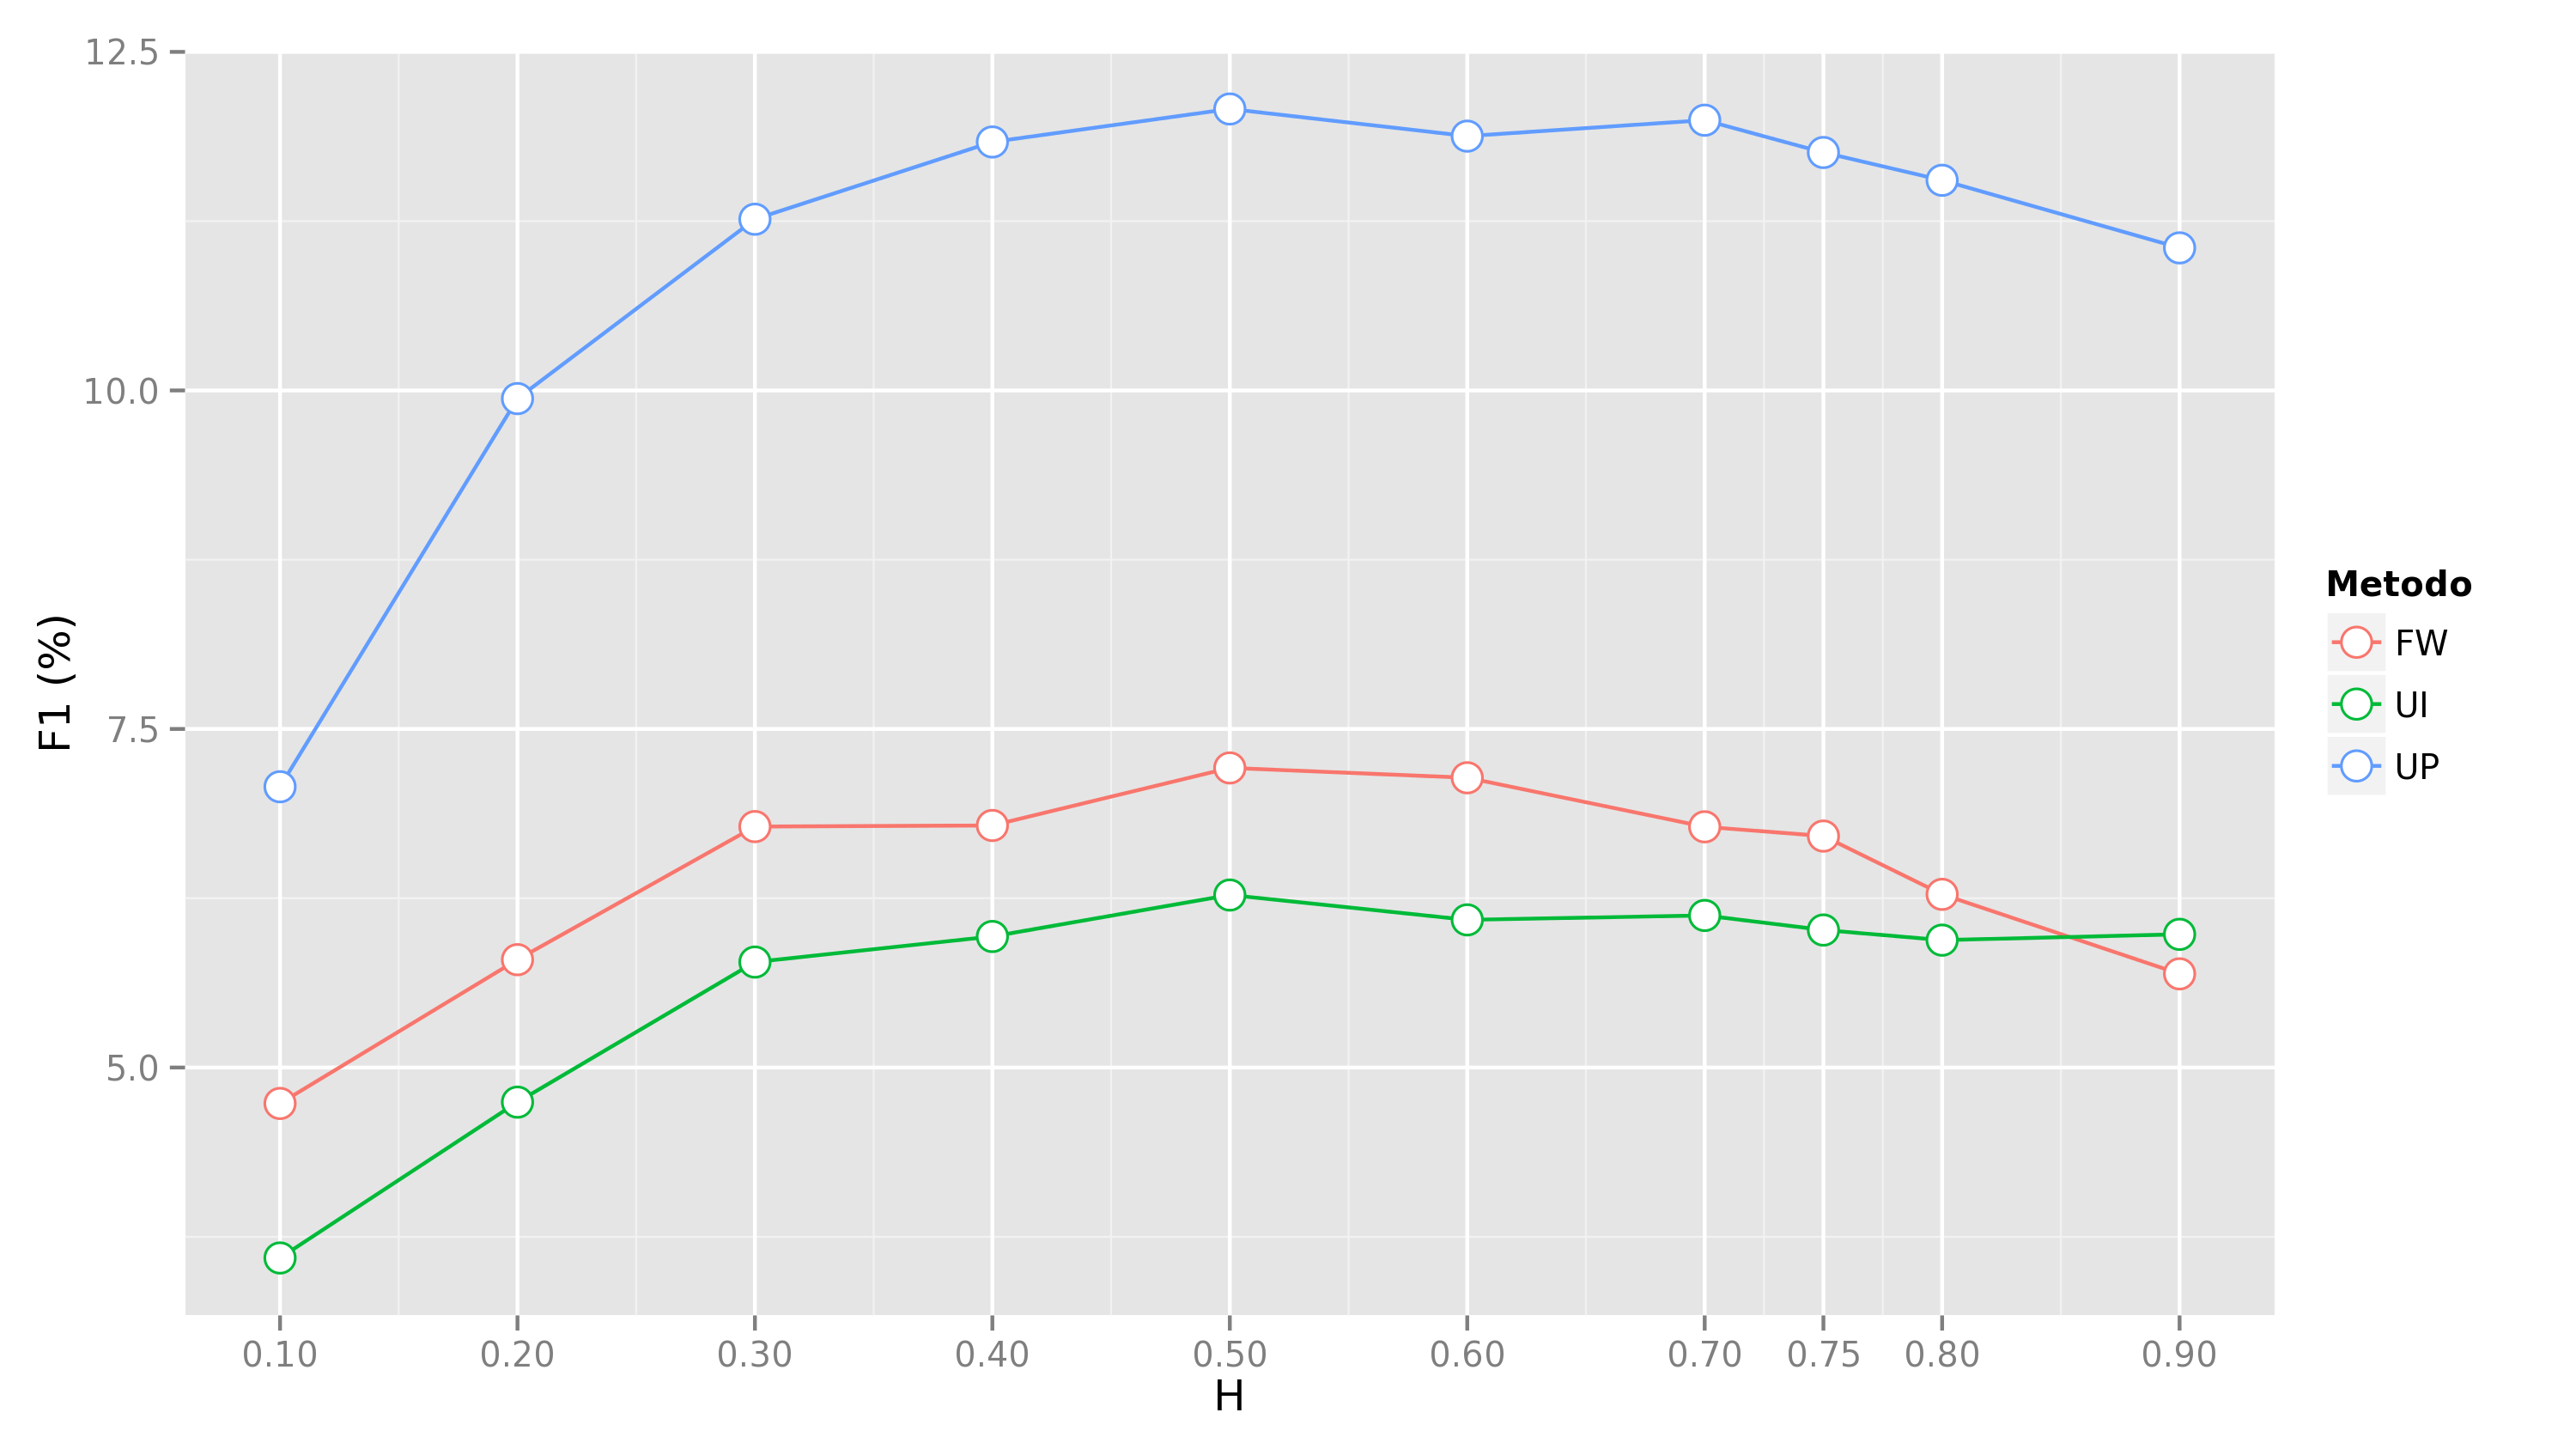
\includegraphics[width=.8\textwidth]{../img/F1_H}
    \end{center}
    \caption{$F_1$ $\times$ $H$}
    \label{fig:F1_H}
\end{figure}
\begin{center}
    Precisão cresce e Abrangência decresce
\end{center}
\end{frame}


\begin{frame}{Resultados}{Medida de distância entre atributos $d^f$}
\begin{figure}[ht]
    \begin{center}
    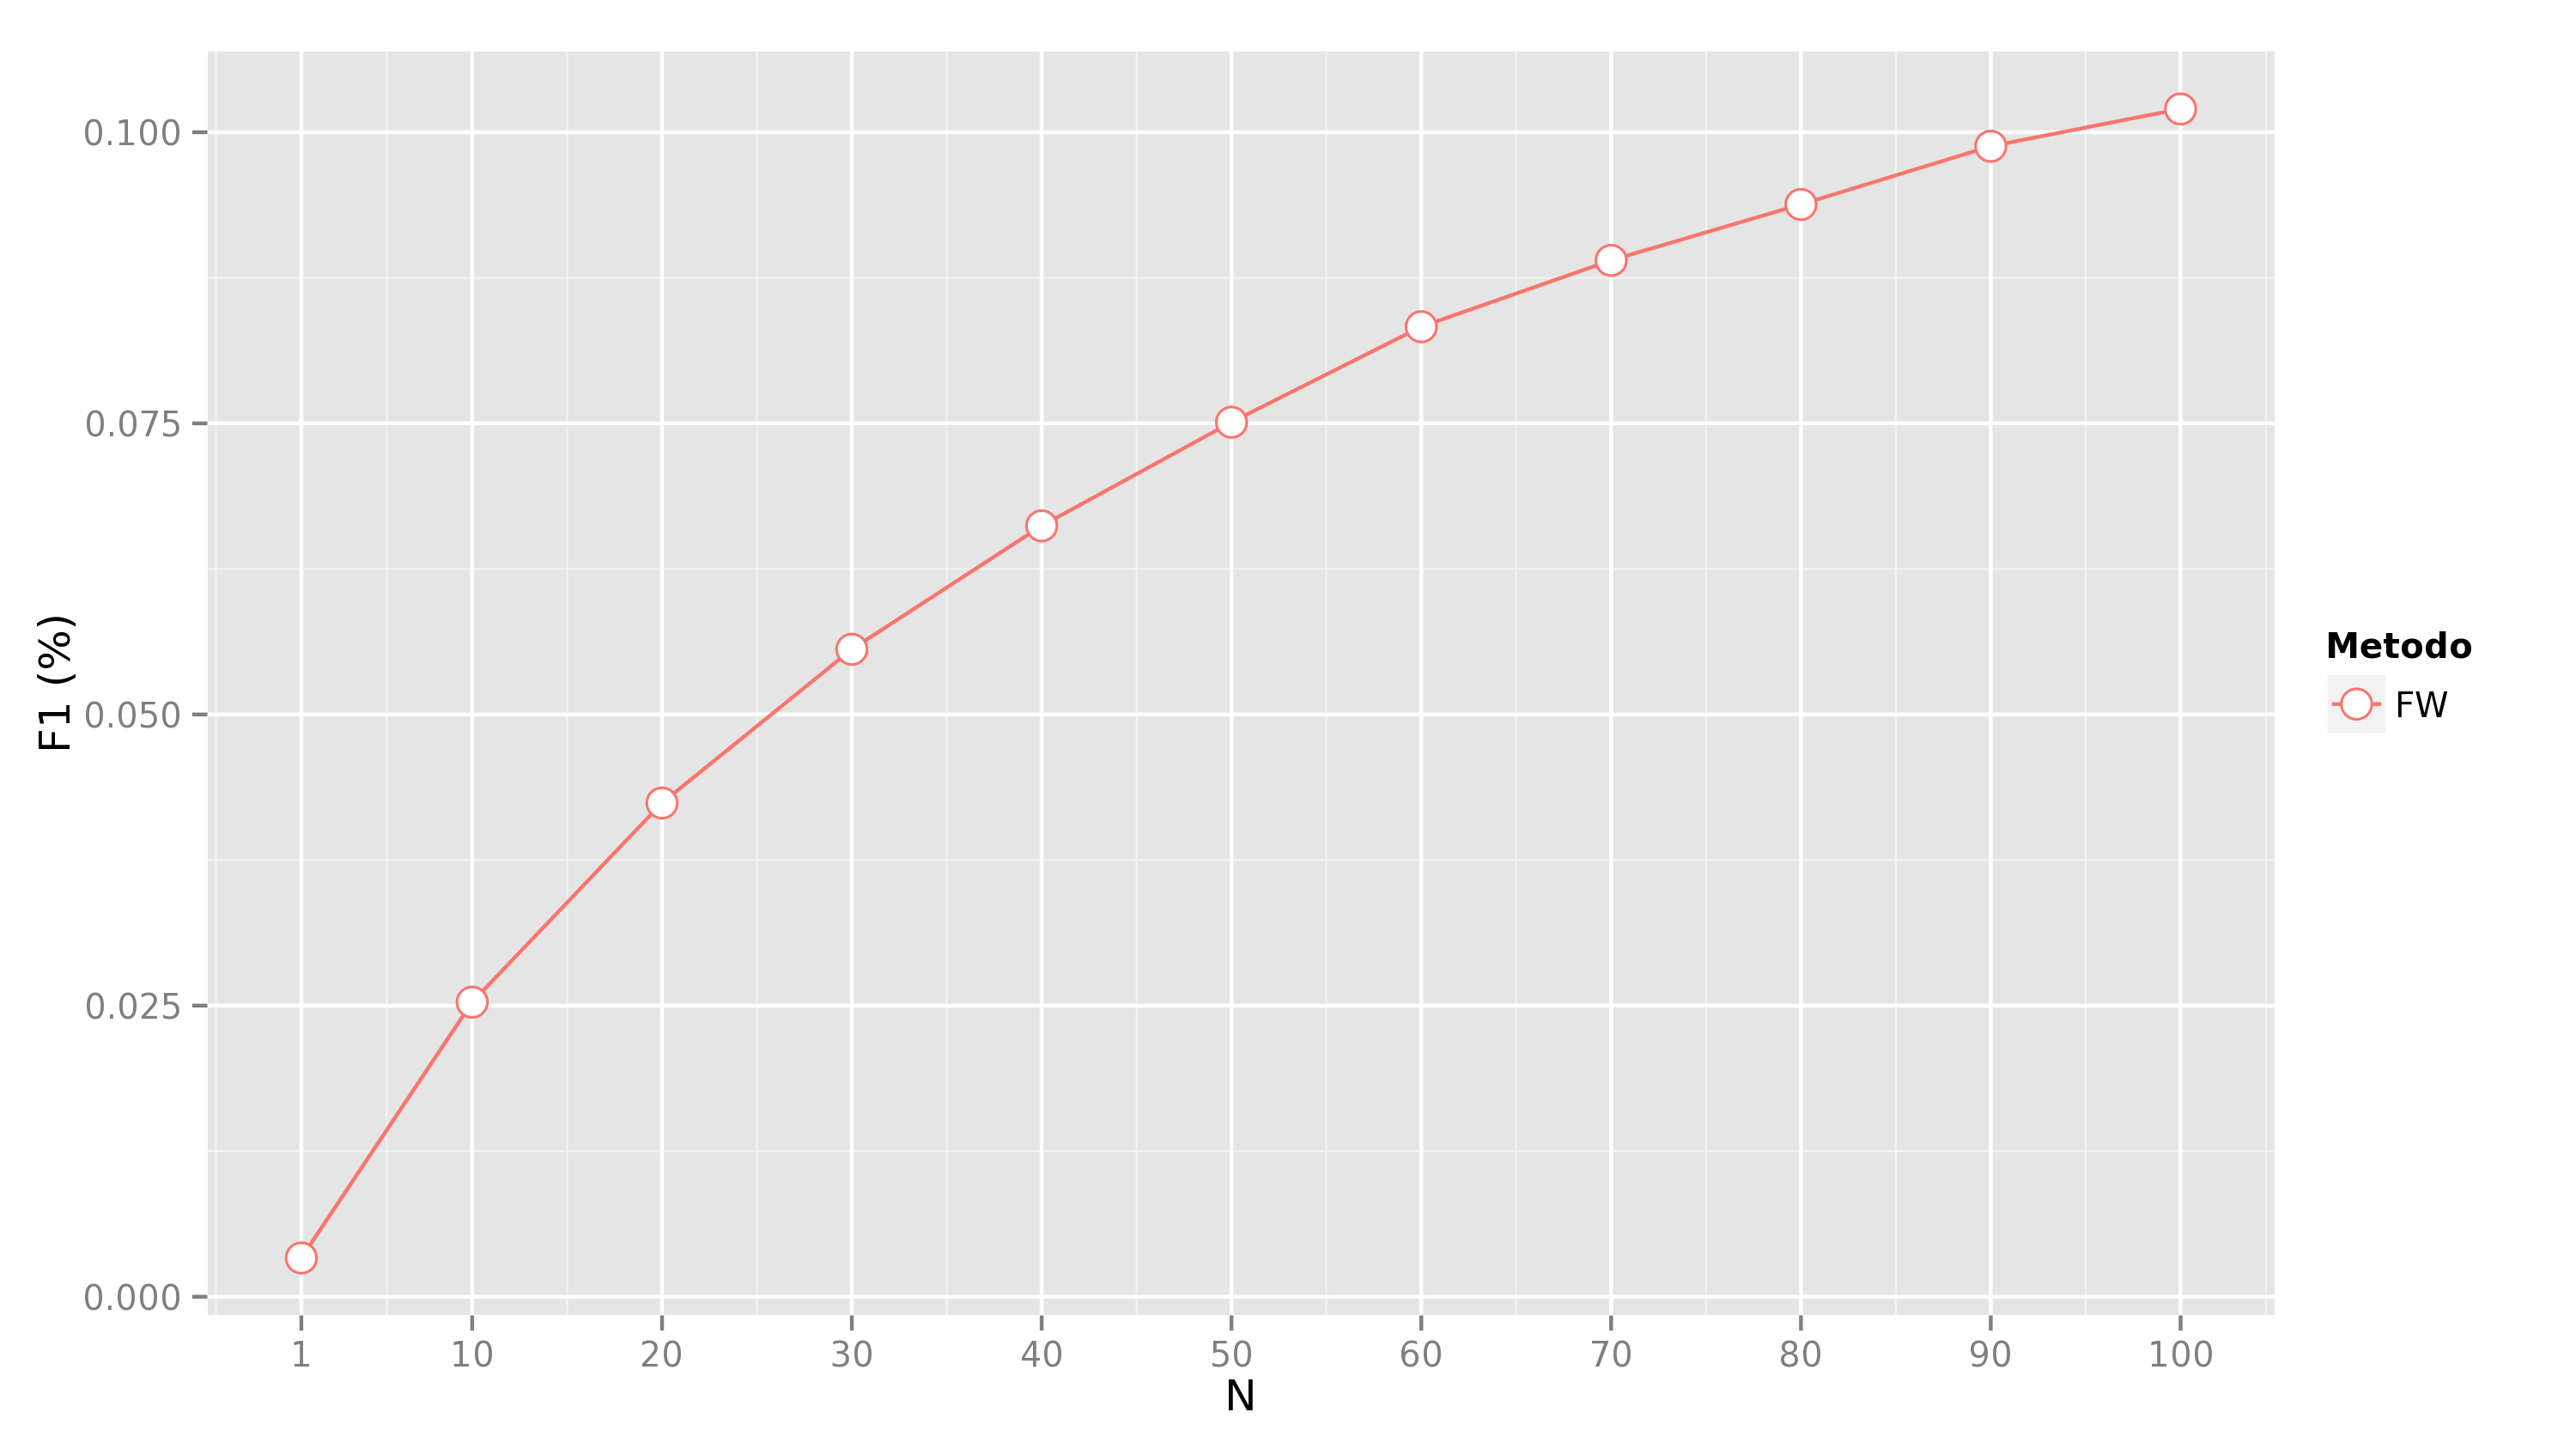
\includegraphics[width=.8\textwidth]{../img/F1_N_d}
    \end{center}
    \caption{$F_1$ $\times$ diferentes $d^f$}
    \label{fig:F1_N_d}
\end{figure}
\begin{center}
    Precisão e Abrangência diminuem com $d^f=J(A,B) ={{|A \cap B|}\over{|A \cup B|}}$
\end{center}
\end{frame}

\begin{frame}{Resultados}{Conjunto de atributos dos itens  $\mathcal{F}$}
\begin{figure}[ht]
    \begin{center}
    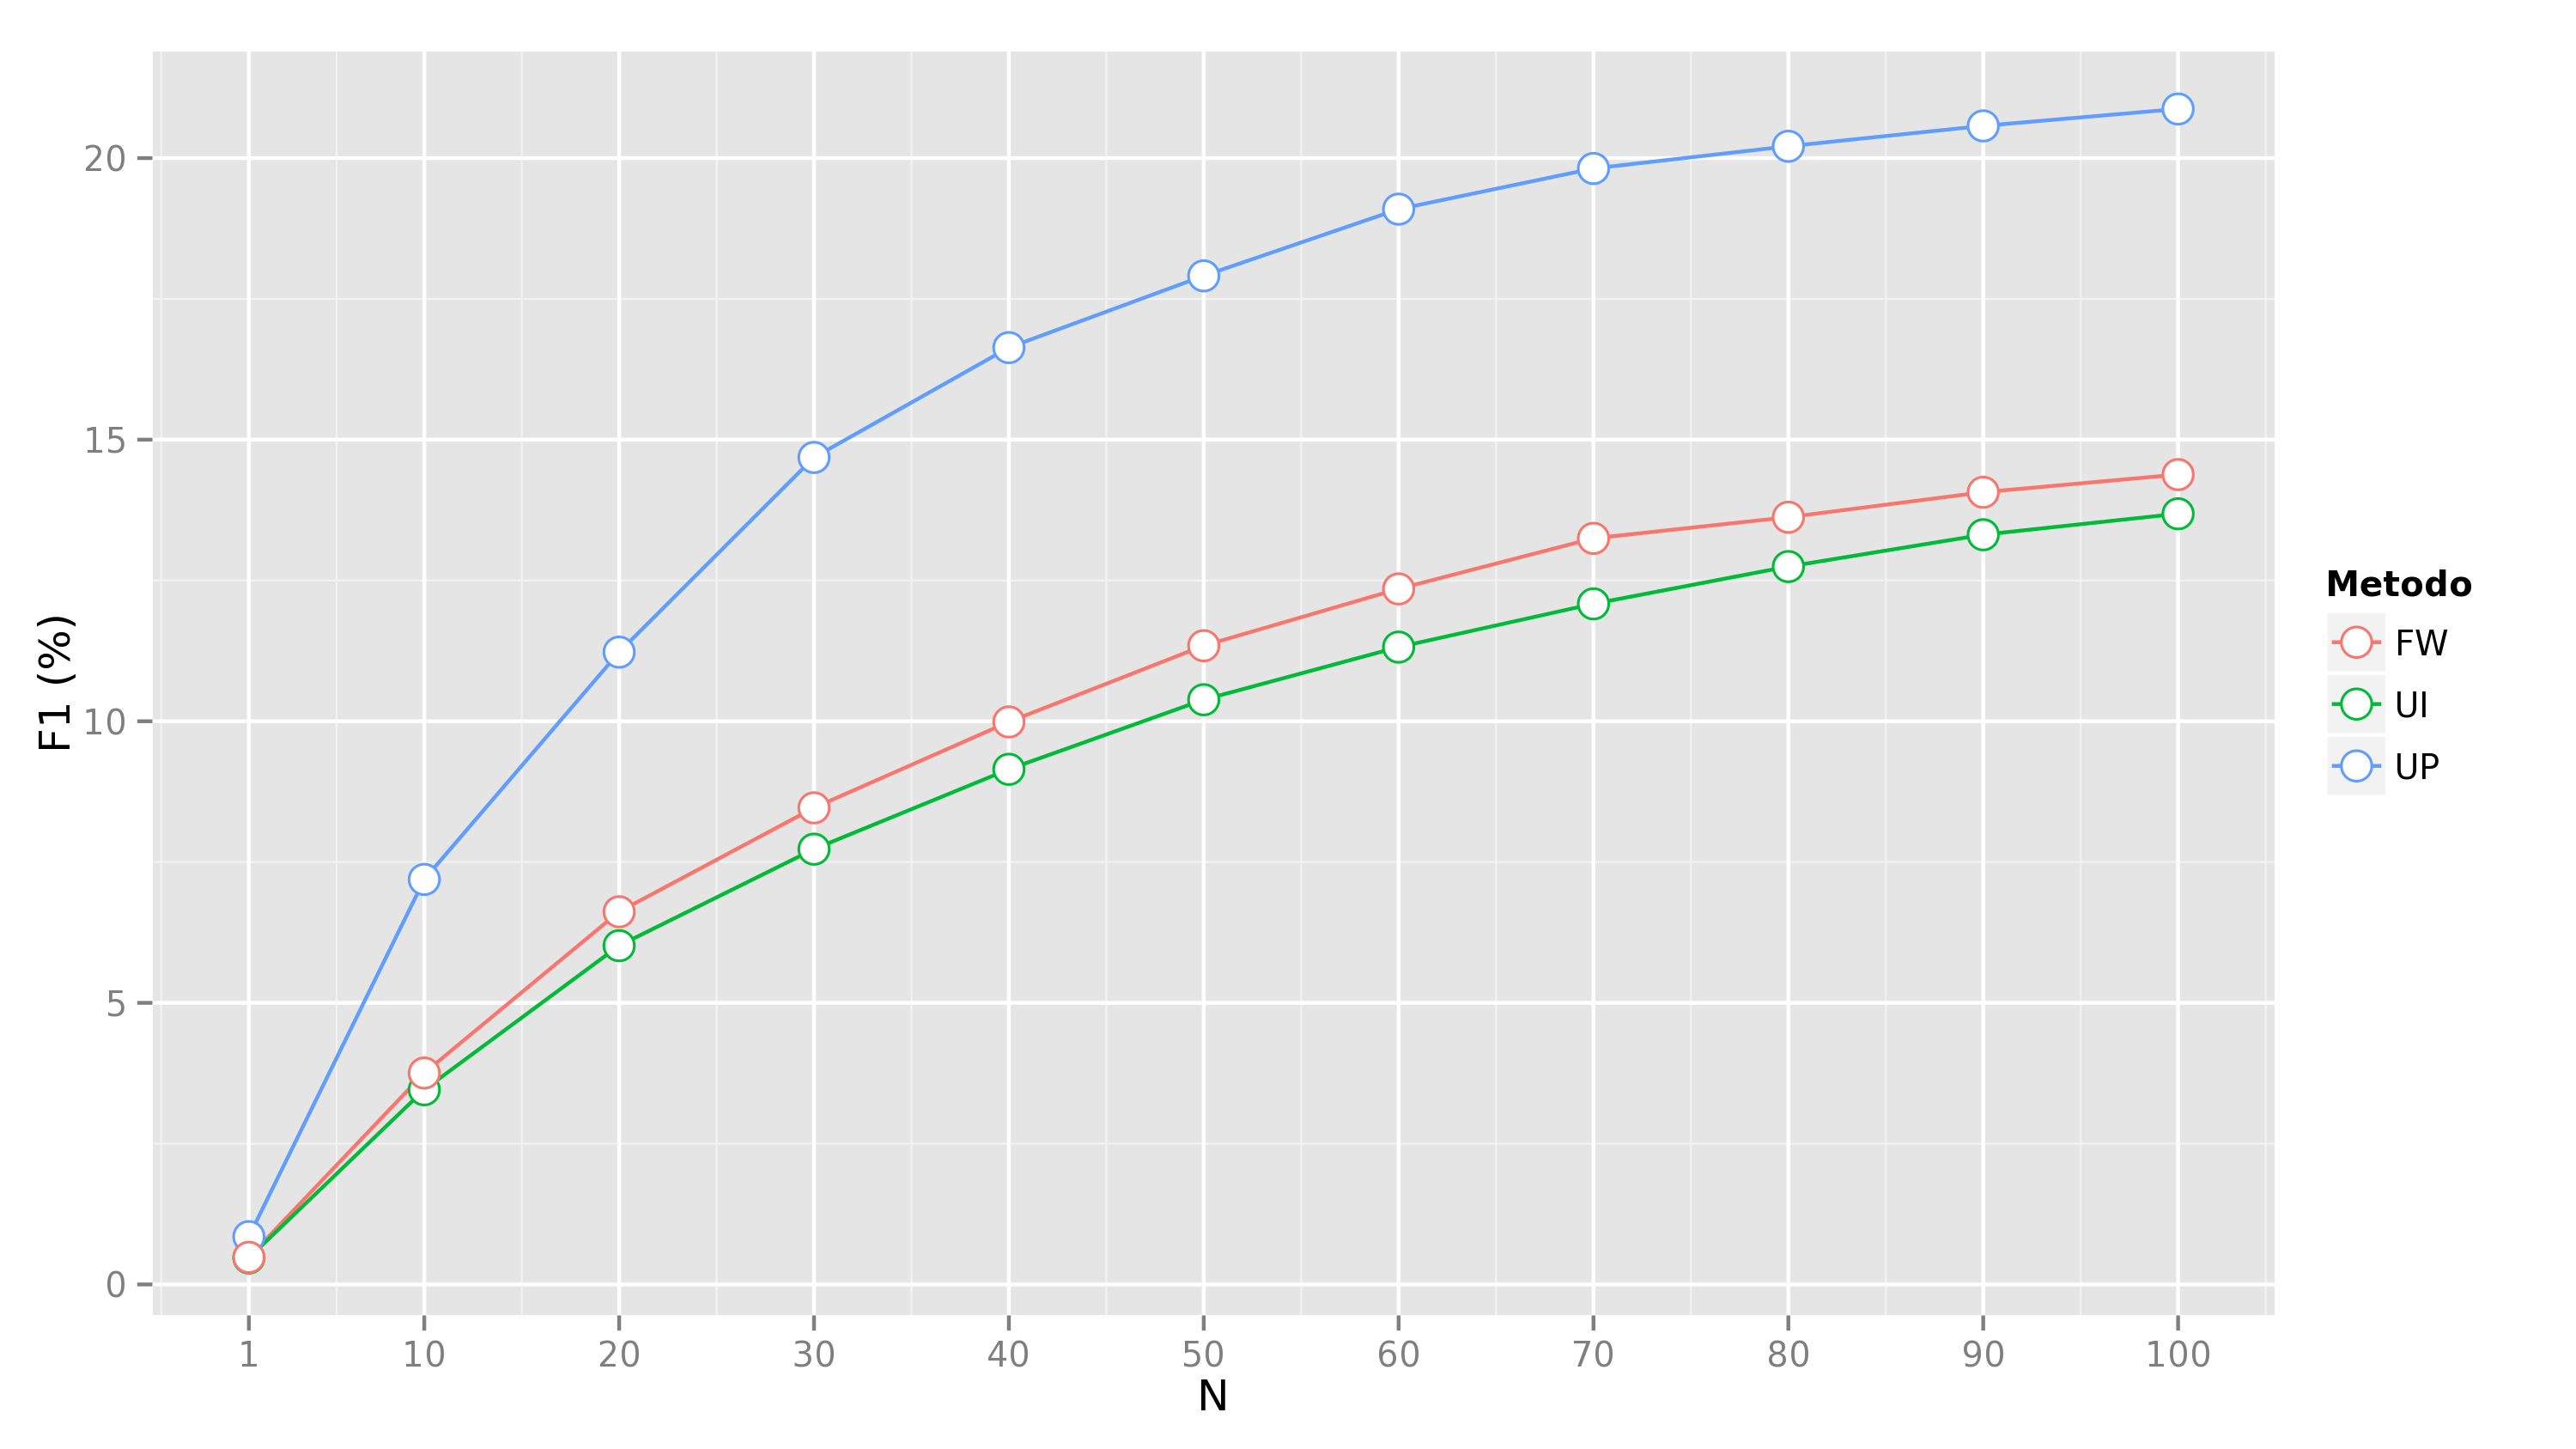
\includegraphics[width=.8\textwidth]{../img/F1_N_F}
    \end{center}
    \caption{$F_1$ $\times$ $\mathcal{F}$}
    \label{fig:F1_N_F}
\end{figure}
\begin{center}
    Precisão e Abrangência aumentam com remoção dos atributos \{data de lançamento, ano\}
\end{center}
\end{frame}




\begin{frame}{Resultados}{$M$, $k$, $W$}
\begin{columns}[b]
\column{.333\textwidth} %
\begin{figure}[ht]
    \begin{center}
    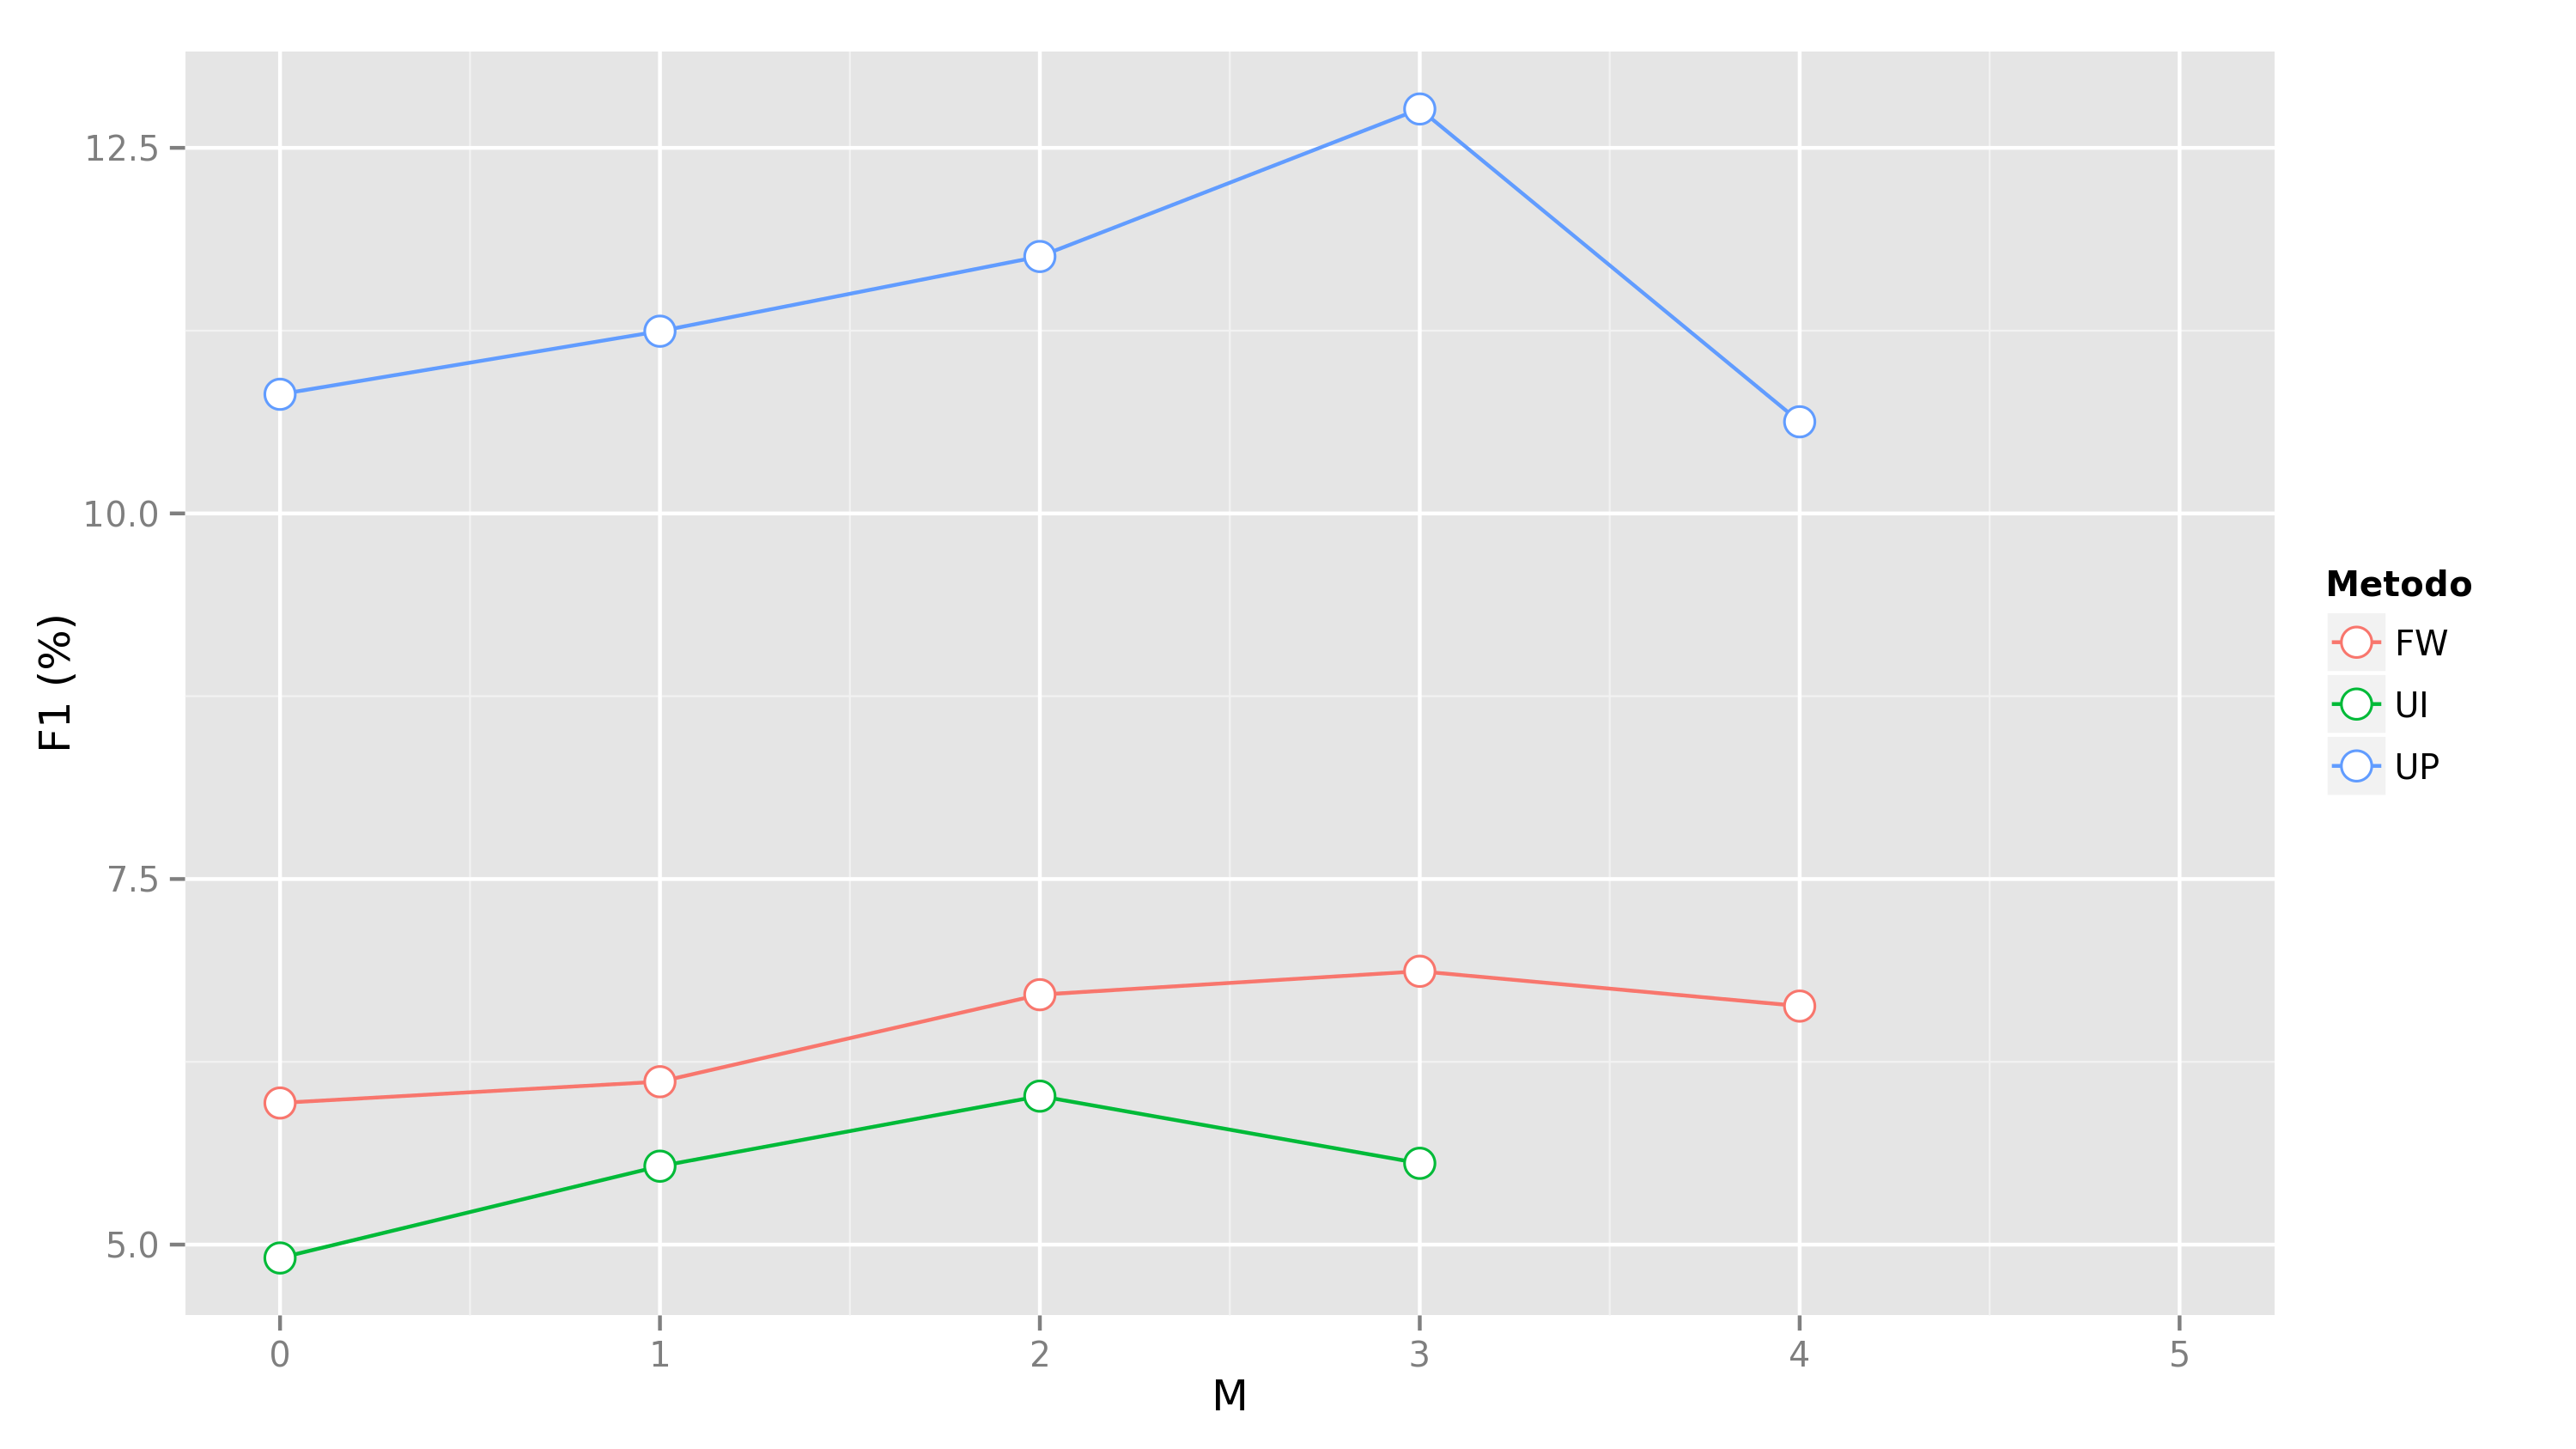
\includegraphics[width=1.1\textwidth]{../img/F1_M}
    \end{center}
    \caption{$F_1$ $\times$ $M$}
    \label{fig:F1_M}
\end{figure}

%Número de vizinhos mais próximos $k$
\column{.333\textwidth} % 
\begin{figure}[ht]
    \begin{center}
    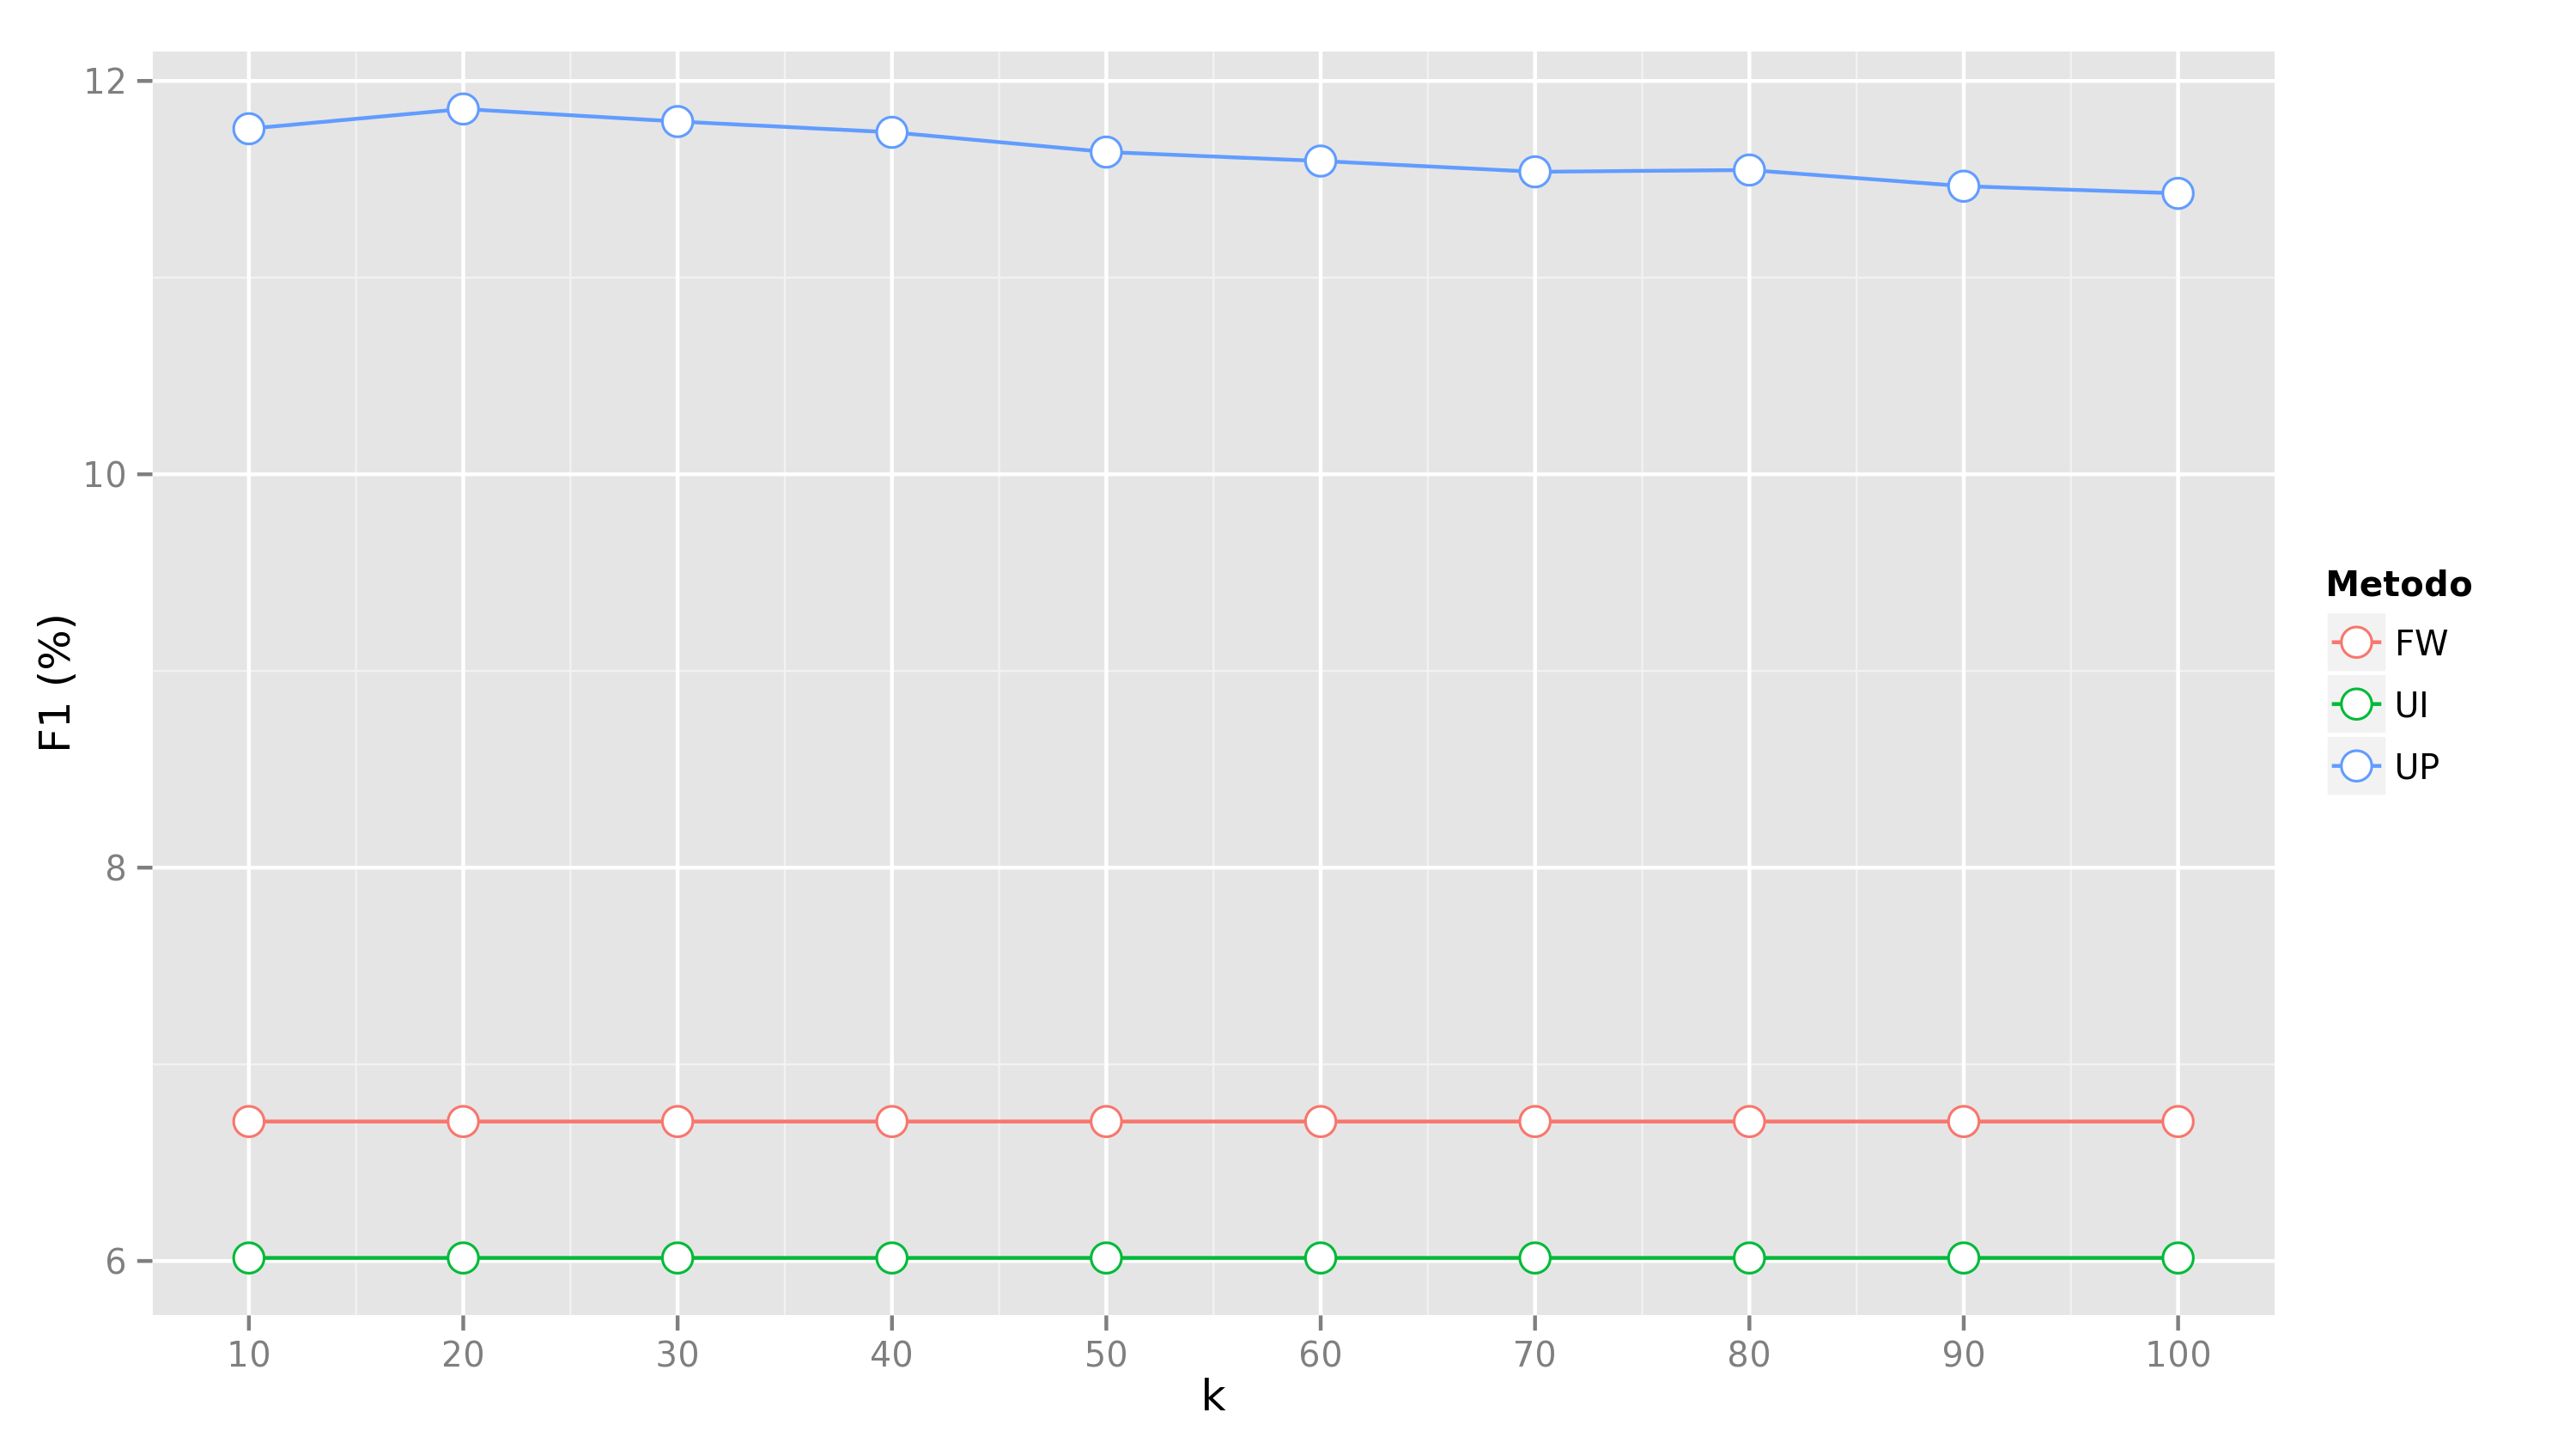
\includegraphics[width=1.1\textwidth]{../img/F1_k}
    \end{center}
    \caption{$F_1$ $\times$ $k$}
    \label{fig:F1_H}
\end{figure}
\column{.333\textwidth} % 

\begin{figure}[ht]
    \begin{center}
    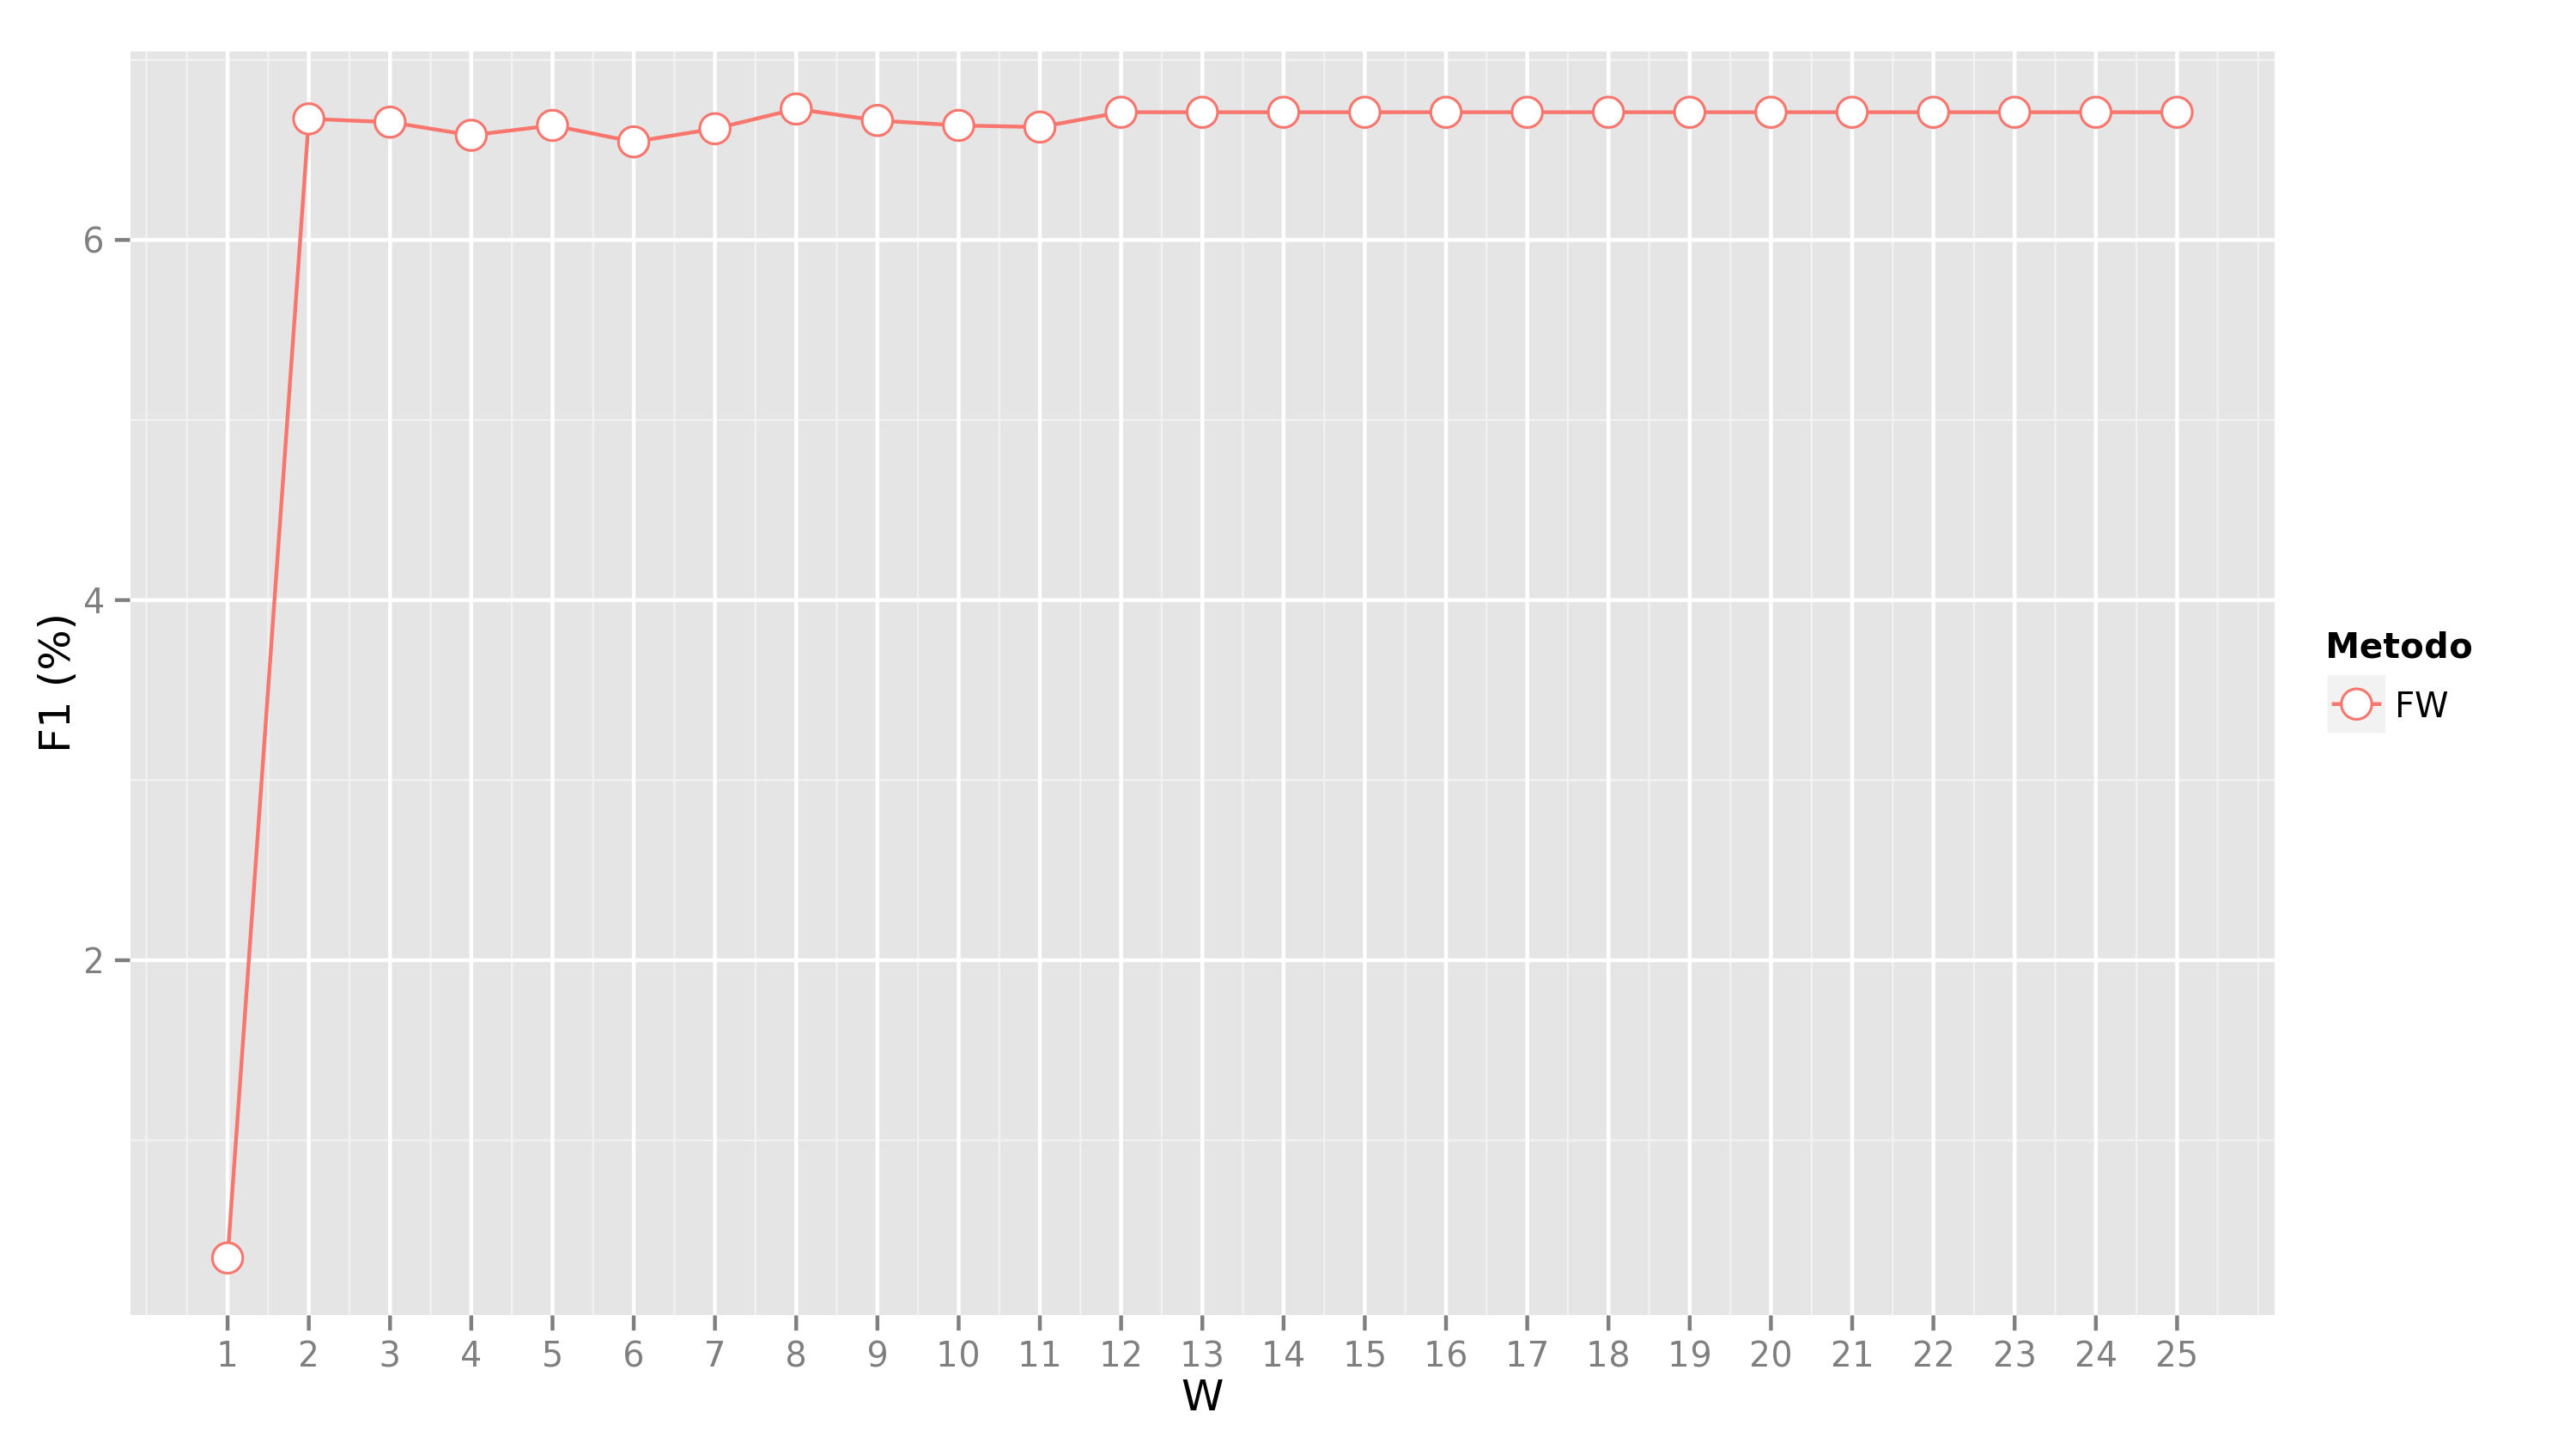
\includegraphics[width=1.1\textwidth]{../img/F1_W}
    \end{center}
    \caption{$F_1$ $\times$ $W$}
    \label{fig:F1_W}
\end{figure}
\end{columns}
\begin{center}
    Precisão e Abrangência praticamente constantes
\end{center}
\end{frame}



%\begin{figure}[ht]
%    \begin{center}
    %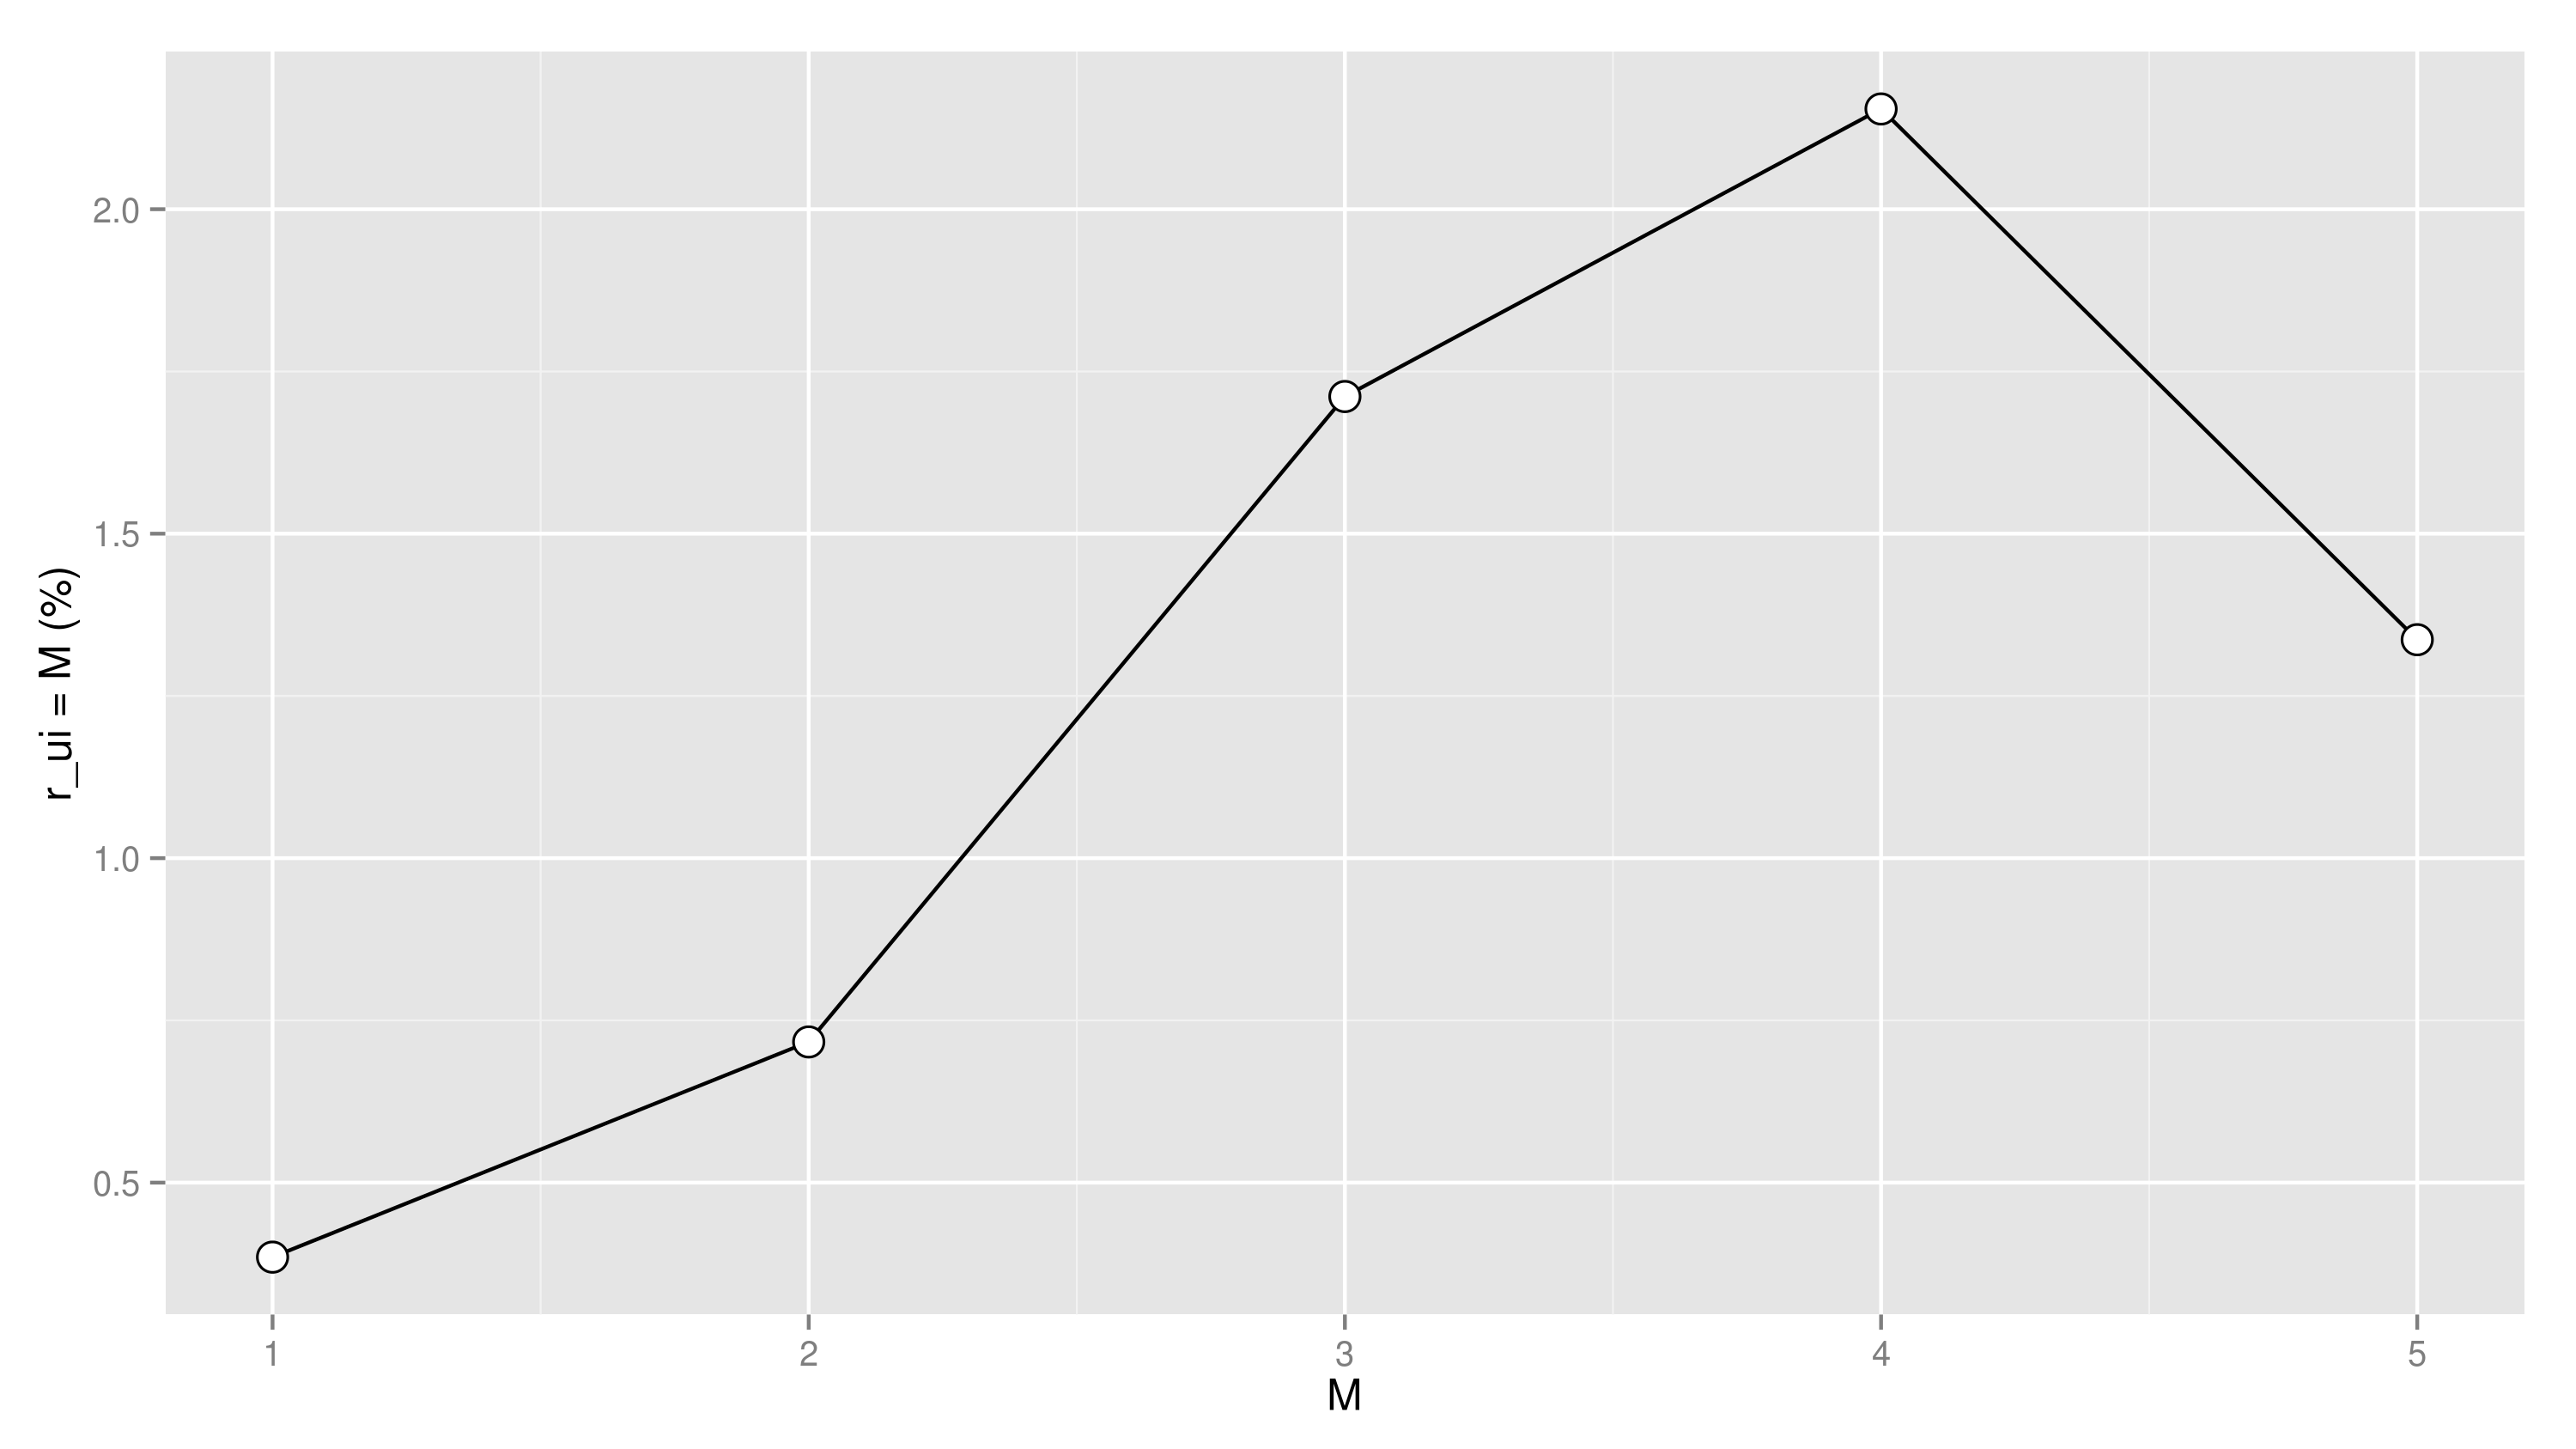
\includegraphics[width=1.1\textwidth]{../img/percentual_M}
%    \end{center}
%    \caption{\{\% $r_{ui} = M$\} $\times$ $M$}
%    \label{fig:percentual_M}
%\end{figure}
